% Seminarul 10: VaR, ES și backtesting
% Statistica piețelor financiare -- Program de licență, Academia de Studii Economice din București
% GENERAT de latex/build_seminar10.py -- modificați generatorul, nu acest fișier.
% Implicit versiunea pentru studenți; versiunea profesorului este wrapper-ul *_solutions.tex.
\makeatletter\@ifundefined{ifsolutions}{\expandafter\newif\csname ifsolutions\endcsname}{}\makeatother

\newcommand{\coursename}{Statistica piețelor financiare}
\def\sfmlang{ro}
% Preambul comun SFM -- Statistica piețelor financiare / Statistics of Financial Markets (Beamer, 16:9)
% Același design ca MFM. Înainte de % Preambul comun SFM -- Statistica piețelor financiare / Statistics of Financial Markets (Beamer, 16:9)
% Același design ca MFM. Înainte de % Preambul comun SFM -- Statistica piețelor financiare / Statistics of Financial Markets (Beamer, 16:9)
% Același design ca MFM. Înainte de \input{../../latex/preamble} se definește
%   \newcommand{\coursename}{Statistics of Financial Markets}      (EN)
%   \newcommand{\coursename}{Statistica piețelor financiare}       (RO)  și  \def\sfmlang{ro}
% Fișierele .tex se află în EN/Courses, EN/Seminars, RO/Cursuri, RO/Seminarii (două niveluri sub rădăcină).
% Deck-urile sînt generate de latex/build_chapterN.py / build_seminarN.py (vezi latex/sfm_build.py).

\documentclass[9pt, aspectratio=169, t]{beamer}
\providecommand{\coursename}{Statistics of Financial Markets}

% Ensure content fits on slides
\setbeamersize{text margin left=8mm, text margin right=8mm}

%=============================================================================
% THEME AND STYLE CONFIGURATION
%=============================================================================
\usetheme{default}
% Using default theme for clean header/footer control

% Color Palette (matching Redispatch PDF)
\definecolor{MainBlue}{RGB}{26, 58, 110}
\definecolor{AccentBlue}{RGB}{26, 58, 110}
\definecolor{IDAred}{RGB}{205, 0, 0}
\definecolor{DarkGray}{RGB}{51, 51, 51}
\definecolor{MediumGray}{RGB}{128, 128, 128}
\definecolor{LightGray}{RGB}{248, 248, 248}
\definecolor{VeryLightGray}{RGB}{235, 235, 235}
\definecolor{KeynoteGray}{RGB}{218, 218, 218}
\definecolor{SectionGray}{RGB}{120, 120, 120}
\definecolor{FooterGray}{RGB}{100, 100, 100}
\definecolor{Crimson}{RGB}{220, 53, 69}
\definecolor{Forest}{RGB}{46, 125, 50}
\definecolor{Amber}{RGB}{181, 133, 63}
\definecolor{Orange}{RGB}{230, 126, 34}
\definecolor{Purple}{RGB}{142, 68, 173}

% Gradient background (exact Keynote 315° gradient: white to RGB 218,218,218)
\setbeamertemplate{background}{%
    \begin{tikzpicture}[remember picture, overlay]
        \shade[shading=axis, shading angle=315,
        top color=white, bottom color=KeynoteGray]
        (current page.south west) rectangle (current page.north east);
    \end{tikzpicture}%
}
% Fallback solid color for compatibility
\setbeamercolor{background canvas}{bg=}

\setbeamercolor{palette primary}{bg=MainBlue, fg=white}
\setbeamercolor{palette secondary}{bg=MainBlue!85, fg=white}
\setbeamercolor{palette tertiary}{bg=MainBlue!70, fg=white}
\setbeamercolor{structure}{fg=MainBlue}
\setbeamercolor{title}{fg=IDAred}
\setbeamercolor{frametitle}{fg=IDAred, bg=}
\setbeamercolor{block title}{bg=MainBlue, fg=white}
\setbeamercolor{block body}{bg=VeryLightGray, fg=DarkGray}
\setbeamercolor{block title alerted}{bg=Crimson, fg=white}
\setbeamercolor{block body alerted}{bg=Crimson!8, fg=DarkGray}
\setbeamercolor{block title example}{bg=Forest, fg=white}
\setbeamercolor{block body example}{bg=Forest!8, fg=DarkGray}
\setbeamercolor{item}{fg=MainBlue}

% Footer colors (override Madrid theme blue)
\setbeamercolor{author in head/foot}{fg=FooterGray, bg=}
\setbeamercolor{title in head/foot}{fg=FooterGray, bg=}
\setbeamercolor{date in head/foot}{fg=FooterGray, bg=}
\setbeamercolor{section in head/foot}{fg=FooterGray, bg=}
\setbeamercolor{subsection in head/foot}{fg=FooterGray, bg=}

% Bullet styles (apply everywhere including blocks)
\setbeamertemplate{itemize item}{\color{MainBlue}$\boxdot$}
\setbeamertemplate{itemize subitem}{\color{MainBlue}$\blacktriangleright$}
\setbeamertemplate{itemize subsubitem}{\color{MainBlue}\tiny$\bullet$}
\setbeamertemplate{itemize/enumerate body begin}{\normalsize}
\setbeamertemplate{itemize/enumerate subbody begin}{\normalsize}

% Item spacing - compact style
\setlength{\leftmargini}{10pt}       % Level 1: minimal indent
\setlength{\leftmarginii}{10pt}      % Level 2: minimal additional indent
% Compact list spacing (zero extra space before/after lists in blocks)
\makeatletter
\def\@listi{\leftmargin\leftmargini \topsep 0pt \parsep 0pt \itemsep 0pt}
\def\@listii{\leftmargin\leftmarginii \topsep 0pt \parsep 0pt \itemsep 0pt}
\makeatother

\setbeamertemplate{navigation symbols}{}

%=============================================================================
% CUSTOM HEADLINE
%=============================================================================
\setbeamertemplate{headline}{%
    \vskip10pt%
    \hbox to \paperwidth{%
        \hskip0.5cm%
        {\small\color{FooterGray}\renewcommand{\hyperlink}[2]{##2}\insertsectionhead}%
        \hfill%
        \textcolor{FooterGray}{\small\insertframenumber}%
        \hskip0.5cm%
    }%
    \vskip4pt%
    {\color{FooterGray}\hrule height 0.4pt}%
}

%=============================================================================
% CUSTOM FOOTER
%=============================================================================
\usepackage{fontawesome5}

\setbeamertemplate{footline}{%
    {\color{FooterGray}\hrule height 0.4pt}%
    \vskip4pt%
    \hbox to \paperwidth{%
        \hskip0.5cm%
        \textcolor{FooterGray}{\small\coursename}%
        \hfill%
        \raisebox{-0.1em}{%
            \begin{tikzpicture}[x=0.08em, y=0.08em, line width=0.4pt]
                \draw[FooterGray] (0,3) -- (1,4) -- (2,3.5) -- (3,5) -- (4,4) -- (5,6) -- (6,5.5) -- (7,4) -- (8,5) -- (9,7) -- (10,6) -- (11,5) -- (12,6.5) -- (13,8) -- (14,7) -- (15,6) -- (16,7.5) -- (17,9) -- (18,8) -- (19,7) -- (20,8.5) -- (21,10) -- (22,9) -- (23,8) -- (24,9.5);
            \end{tikzpicture}%
        }%
        \hskip0.5cm%
    }%
    \vskip6pt%
}

%=============================================================================
% PACKAGES
%=============================================================================
\usepackage[utf8]{inputenc}
\DeclareUnicodeCharacter{03B1}{\ensuremath{\alpha}}
\usepackage[T1]{fontenc}
\usepackage{amsmath, amssymb, amsthm}
\usepackage{mathtools}
\usepackage{bm}
\usepackage{tikz}
\usetikzlibrary{arrows.meta, positioning, shapes, calc, decorations.pathreplacing, shadings}
\usepackage{booktabs}
\usepackage{multirow}
\usepackage{array}
\usepackage{graphicx}
\usepackage{hyperref}
\usepackage{colortbl}
\usepackage{listings}
\lstset{language=Python, basicstyle=\ttfamily\scriptsize, keywordstyle=\color{MainBlue}\bfseries,
  commentstyle=\color{Forest}, stringstyle=\color{Crimson}, breaklines=true,
  frame=none, backgroundcolor=\color{VeryLightGray}, xleftmargin=2mm}
\hypersetup{colorlinks=true, linkcolor=MainBlue, urlcolor=MainBlue}
\graphicspath{{../../logos/}{../../charts/}{../../photos/}}
\usepackage{xcolor}
\hfuzz=2pt  % Suppress tiny overfull warnings (<2pt)
\vfuzz=2pt  % Suppress tiny vertical overfull warnings (<2pt)

%=============================================================================
% QUANTLET COMMANDS
%   \quantlet{<displayed name>}{<url>}       (generic, compatible with the older SFM decks)
%   \sfmquantlet{Ch_05}{SFM_ch5_garch}       -> https://github.com/danpele/SFM/tree/main/Quantlets/Ch_05/SFM_ch5_garch
%   \qlurl{<folder>} is defined per chapter by the generator (Quantlets/Ch_NN/<folder>)
%=============================================================================
\newcommand{\sfmrepo}{https://github.com/danpele/SFM}
\newcommand{\sfmqlbase}{https://github.com/danpele/SFM/tree/main/Quantlets}
\newcommand{\quantlet}[2]{%
    \hfill\href{#2}{%
        \raisebox{-0.15em}{
\includegraphics[height=0.7em]{ql_logo.png}}%
        \textcolor{MainBlue}{\tiny\ #1}%
    }%
}
\newcommand{\sfmquantlet}[2]{\quantlet{\detokenize{#2}}{\sfmqlbase/#1/#2}}

%=============================================================================
% NOTEBOOKS (Google Colab)
%   \colaburl{notebooks/EN/chapter5_seminar_notebook.ipynb} -> the Colab link of a file in the SFM repo
%   \nb: the chapter notebook (each seminar deck redefines it with \renewcommand)
%=============================================================================
\newcommand{\colaburl}[1]{https://colab.research.google.com/github/danpele/SFM/blob/main/#1}
\newcommand{\nb}{https://colab.research.google.com/github/danpele/SFM/tree/main/notebooks/EN}
\newcommand{\nbname}{notebooks/EN}

%=============================================================================
% SLIDE HELPERS (used by the generators; the same as in MFM)
%=============================================================================
% local font size for list bodies (the preamble forces \normalsize)
\newcommand{\itemsize}[1]{\setbeamertemplate{itemize/enumerate body begin}{#1}\setbeamertemplate{itemize/enumerate subbody begin}{#1}}
\newcommand{\intitle}[1]{{\hypersetup{urlcolor=white}#1}}   % white links inside coloured title bars
\newcommand{\imgcap}[1]{{\scriptsize #1}\\[0.5mm]}          % caption under a photo
\newcommand{\imgcredit}[2]{{\tiny\color{FooterGray}\href{#1}{#2}}}   % image credit: source URL, author/licence
\newcommand{\aiprompt}[1]{{\ttfamily\color{MainBlue}#1}}     % a prompt to an AI assistant

%=============================================================================
% SEMINARS: student version by default; the instructor wrapper *_solutions.tex sets \solutionstrue
%=============================================================================
\makeatletter\@ifundefined{ifsolutions}{\expandafter\newif\csname ifsolutions\endcsname}{}\makeatother
\newcommand{\solonly}[1]{\ifsolutions #1\fi}
\newcommand{\propsub}{\ifsolutions\else\framesubtitle{\ifdefined\sfmlang Rezolvarea se discută la seminar\else Solution discussed in class\fi}\fi}

%=============================================================================
% APPENDIX AND CHAPTER LINKS (latex/appendix_links.py writes the calls; it also re-declares these
% macros before \begin{document}, so the decks compile with or without this preamble block)
%=============================================================================
\providecommand{\sfmapplink}[3]{\hypertarget{#2}{}\hyperlink{#1}{\beamergotobutton{#3}}}
\providecommand{\sfmappback}[2]{\begin{tikzpicture}[remember picture,overlay]\node[anchor=south east] at ([xshift=-3mm,yshift=7mm]current page.south east){\hyperlink{#1}{\beamerreturnbutton{#2}}};\end{tikzpicture}}
\providecommand{\sfmchlink}[2]{\href{#1}{#2}}
\providecommand{\sfmchlinkt}[2]{\href{#1}{\usebeamercolor[fg]{frametitle}#2}}

%=============================================================================
% QUANTINAR COMMAND: link către un curs Quantinar (subiecte avansate)
%=============================================================================
\newcommand{\quantinar}[2]{%
    \href{#2}{%
        \raisebox{-0.15em}{
\includegraphics[height=0.8em]{qr_logo.png}}%
        \textcolor{MainBlue}{\scriptsize\ #1}%
    }%
}

%=============================================================================
% CUSTOM TITLE PAGE
%=============================================================================
\defbeamertemplate*{title page}{hybrid}[1][]
{
    \vspace{0.2cm}
    % Logos row - top header (with clickable links)
    \begin{center}
        \href{https://www.ase.ro}{
\includegraphics[height=1.0cm]{ase_logo.png}}\hspace{0.3cm}%
        \href{https://theida.net}{
\includegraphics[height=1.0cm]{ida_logo.png}}\hspace{0.3cm}%
        \href{https://blockchain-research-center.com}{
\includegraphics[height=1.0cm]{brc_logo.png}}\hspace{0.3cm}%
        \href{https://www.ai4efin.ase.ro}{
\includegraphics[height=1.0cm]{ai4efin_logo.png}}\hspace{0.3cm}%
        \href{https://ipe.ro/new}{
\includegraphics[height=1.0cm]{acad_logo.png}}\hspace{0.3cm}%
        \href{https://www.digital-finance-msca.com}{
\includegraphics[height=1.0cm]{msca_logo.png}}%
    \end{center}

    \vspace{0.6cm}

    % Main title with Q logos on sides (with clickable links)
    \begin{center}
        \begin{minipage}{0.1\textwidth}
            \centering
            \href{https://quantlet.com}{
\includegraphics[height=1.1cm]{ql_logo.png}}
        \end{minipage}%
        \begin{minipage}{0.78\textwidth}
            \centering
            {\LARGE\bfseries\usebeamercolor[fg]{title}\inserttitle}

            \vspace{0.3cm}

            {\usebeamerfont{subtitle}\usebeamercolor[fg]{title}\insertsubtitle}
        \end{minipage}%
        \begin{minipage}{0.1\textwidth}
            \centering
            \href{https://quantinar.com}{
\includegraphics[height=1.1cm]{qr_logo.png}}
        \end{minipage}
    \end{center}

    \vspace{0.6cm}

    % Authors (left aligned)
    \hspace{0.5cm}{\usebeamerfont{author}\insertauthor}

    \vspace{0.3cm}

    % Institute/Affiliations (left aligned)
    \hspace{0.5cm}\begin{minipage}[t]{0.9\textwidth}
        \raggedright\small\insertinstitute
    \end{minipage}
}

%=============================================================================
% THEOREM ENVIRONMENTS
%=============================================================================
\theoremstyle{definition}
\setbeamertemplate{theorems}[numbered]
\ifdefined\sfmlang
\newtheorem{defn}{Definiție}
\newtheorem{thm}{Teoremă}
\newtheorem{prop}{Propoziție}
\newtheorem{rmk}{Observație}
\else
\newtheorem{defn}{Definition}
\newtheorem{thm}{Theorem}
\newtheorem{prop}{Proposition}
\newtheorem{rmk}{Remark}
\fi

%=============================================================================
% CENTRED MINIPAGE (no extra vertical space)
%=============================================================================
\newenvironment{cminipage}[1]{%
    \par\noindent\hfill\begin{minipage}{#1}\ignorespaces
}{%
    \end{minipage}\hfill\null\par
}

%=============================================================================
% CUSTOM COMMANDS
%=============================================================================
\newcommand{\E}{\mathbb{E}}
\newcommand{\Var}{\text{Var}}
\newcommand{\Cov}{\text{Cov}}
\newcommand{\Corr}{\text{Corr}}
\newcommand{\R}{\mathbb{R}}
\newcommand{\N}{\mathbb{N}}
\newcommand{\Z}{\mathbb{Z}}
\newcommand{\B}{\mathbf{B}}
\newcommand{\imark}{\textcolor{MainBlue}{\textbullet}}
\newcommand{\RMSE}{\text{RMSE}}
\newcommand{\MAE}{\text{MAE}}
\newcommand{\MAPE}{\text{MAPE}}

 se definește
%   \newcommand{\coursename}{Statistics of Financial Markets}      (EN)
%   \newcommand{\coursename}{Statistica piețelor financiare}       (RO)  și  \def\sfmlang{ro}
% Fișierele .tex se află în EN/Courses, EN/Seminars, RO/Cursuri, RO/Seminarii (două niveluri sub rădăcină).
% Deck-urile sînt generate de latex/build_chapterN.py / build_seminarN.py (vezi latex/sfm_build.py).

\documentclass[9pt, aspectratio=169, t]{beamer}
\providecommand{\coursename}{Statistics of Financial Markets}

% Ensure content fits on slides
\setbeamersize{text margin left=8mm, text margin right=8mm}

%=============================================================================
% THEME AND STYLE CONFIGURATION
%=============================================================================
\usetheme{default}
% Using default theme for clean header/footer control

% Color Palette (matching Redispatch PDF)
\definecolor{MainBlue}{RGB}{26, 58, 110}
\definecolor{AccentBlue}{RGB}{26, 58, 110}
\definecolor{IDAred}{RGB}{205, 0, 0}
\definecolor{DarkGray}{RGB}{51, 51, 51}
\definecolor{MediumGray}{RGB}{128, 128, 128}
\definecolor{LightGray}{RGB}{248, 248, 248}
\definecolor{VeryLightGray}{RGB}{235, 235, 235}
\definecolor{KeynoteGray}{RGB}{218, 218, 218}
\definecolor{SectionGray}{RGB}{120, 120, 120}
\definecolor{FooterGray}{RGB}{100, 100, 100}
\definecolor{Crimson}{RGB}{220, 53, 69}
\definecolor{Forest}{RGB}{46, 125, 50}
\definecolor{Amber}{RGB}{181, 133, 63}
\definecolor{Orange}{RGB}{230, 126, 34}
\definecolor{Purple}{RGB}{142, 68, 173}

% Gradient background (exact Keynote 315° gradient: white to RGB 218,218,218)
\setbeamertemplate{background}{%
    \begin{tikzpicture}[remember picture, overlay]
        \shade[shading=axis, shading angle=315,
        top color=white, bottom color=KeynoteGray]
        (current page.south west) rectangle (current page.north east);
    \end{tikzpicture}%
}
% Fallback solid color for compatibility
\setbeamercolor{background canvas}{bg=}

\setbeamercolor{palette primary}{bg=MainBlue, fg=white}
\setbeamercolor{palette secondary}{bg=MainBlue!85, fg=white}
\setbeamercolor{palette tertiary}{bg=MainBlue!70, fg=white}
\setbeamercolor{structure}{fg=MainBlue}
\setbeamercolor{title}{fg=IDAred}
\setbeamercolor{frametitle}{fg=IDAred, bg=}
\setbeamercolor{block title}{bg=MainBlue, fg=white}
\setbeamercolor{block body}{bg=VeryLightGray, fg=DarkGray}
\setbeamercolor{block title alerted}{bg=Crimson, fg=white}
\setbeamercolor{block body alerted}{bg=Crimson!8, fg=DarkGray}
\setbeamercolor{block title example}{bg=Forest, fg=white}
\setbeamercolor{block body example}{bg=Forest!8, fg=DarkGray}
\setbeamercolor{item}{fg=MainBlue}

% Footer colors (override Madrid theme blue)
\setbeamercolor{author in head/foot}{fg=FooterGray, bg=}
\setbeamercolor{title in head/foot}{fg=FooterGray, bg=}
\setbeamercolor{date in head/foot}{fg=FooterGray, bg=}
\setbeamercolor{section in head/foot}{fg=FooterGray, bg=}
\setbeamercolor{subsection in head/foot}{fg=FooterGray, bg=}

% Bullet styles (apply everywhere including blocks)
\setbeamertemplate{itemize item}{\color{MainBlue}$\boxdot$}
\setbeamertemplate{itemize subitem}{\color{MainBlue}$\blacktriangleright$}
\setbeamertemplate{itemize subsubitem}{\color{MainBlue}\tiny$\bullet$}
\setbeamertemplate{itemize/enumerate body begin}{\normalsize}
\setbeamertemplate{itemize/enumerate subbody begin}{\normalsize}

% Item spacing - compact style
\setlength{\leftmargini}{10pt}       % Level 1: minimal indent
\setlength{\leftmarginii}{10pt}      % Level 2: minimal additional indent
% Compact list spacing (zero extra space before/after lists in blocks)
\makeatletter
\def\@listi{\leftmargin\leftmargini \topsep 0pt \parsep 0pt \itemsep 0pt}
\def\@listii{\leftmargin\leftmarginii \topsep 0pt \parsep 0pt \itemsep 0pt}
\makeatother

\setbeamertemplate{navigation symbols}{}

%=============================================================================
% CUSTOM HEADLINE
%=============================================================================
\setbeamertemplate{headline}{%
    \vskip10pt%
    \hbox to \paperwidth{%
        \hskip0.5cm%
        {\small\color{FooterGray}\renewcommand{\hyperlink}[2]{##2}\insertsectionhead}%
        \hfill%
        \textcolor{FooterGray}{\small\insertframenumber}%
        \hskip0.5cm%
    }%
    \vskip4pt%
    {\color{FooterGray}\hrule height 0.4pt}%
}

%=============================================================================
% CUSTOM FOOTER
%=============================================================================
\usepackage{fontawesome5}

\setbeamertemplate{footline}{%
    {\color{FooterGray}\hrule height 0.4pt}%
    \vskip4pt%
    \hbox to \paperwidth{%
        \hskip0.5cm%
        \textcolor{FooterGray}{\small\coursename}%
        \hfill%
        \raisebox{-0.1em}{%
            \begin{tikzpicture}[x=0.08em, y=0.08em, line width=0.4pt]
                \draw[FooterGray] (0,3) -- (1,4) -- (2,3.5) -- (3,5) -- (4,4) -- (5,6) -- (6,5.5) -- (7,4) -- (8,5) -- (9,7) -- (10,6) -- (11,5) -- (12,6.5) -- (13,8) -- (14,7) -- (15,6) -- (16,7.5) -- (17,9) -- (18,8) -- (19,7) -- (20,8.5) -- (21,10) -- (22,9) -- (23,8) -- (24,9.5);
            \end{tikzpicture}%
        }%
        \hskip0.5cm%
    }%
    \vskip6pt%
}

%=============================================================================
% PACKAGES
%=============================================================================
\usepackage[utf8]{inputenc}
\DeclareUnicodeCharacter{03B1}{\ensuremath{\alpha}}
\usepackage[T1]{fontenc}
\usepackage{amsmath, amssymb, amsthm}
\usepackage{mathtools}
\usepackage{bm}
\usepackage{tikz}
\usetikzlibrary{arrows.meta, positioning, shapes, calc, decorations.pathreplacing, shadings}
\usepackage{booktabs}
\usepackage{multirow}
\usepackage{array}
\usepackage{graphicx}
\usepackage{hyperref}
\usepackage{colortbl}
\usepackage{listings}
\lstset{language=Python, basicstyle=\ttfamily\scriptsize, keywordstyle=\color{MainBlue}\bfseries,
  commentstyle=\color{Forest}, stringstyle=\color{Crimson}, breaklines=true,
  frame=none, backgroundcolor=\color{VeryLightGray}, xleftmargin=2mm}
\hypersetup{colorlinks=true, linkcolor=MainBlue, urlcolor=MainBlue}
\graphicspath{{../../logos/}{../../charts/}{../../photos/}}
\usepackage{xcolor}
\hfuzz=2pt  % Suppress tiny overfull warnings (<2pt)
\vfuzz=2pt  % Suppress tiny vertical overfull warnings (<2pt)

%=============================================================================
% QUANTLET COMMANDS
%   \quantlet{<displayed name>}{<url>}       (generic, compatible with the older SFM decks)
%   \sfmquantlet{Ch_05}{SFM_ch5_garch}       -> https://github.com/danpele/SFM/tree/main/Quantlets/Ch_05/SFM_ch5_garch
%   \qlurl{<folder>} is defined per chapter by the generator (Quantlets/Ch_NN/<folder>)
%=============================================================================
\newcommand{\sfmrepo}{https://github.com/danpele/SFM}
\newcommand{\sfmqlbase}{https://github.com/danpele/SFM/tree/main/Quantlets}
\newcommand{\quantlet}[2]{%
    \hfill\href{#2}{%
        \raisebox{-0.15em}{
\includegraphics[height=0.7em]{ql_logo.png}}%
        \textcolor{MainBlue}{\tiny\ #1}%
    }%
}
\newcommand{\sfmquantlet}[2]{\quantlet{\detokenize{#2}}{\sfmqlbase/#1/#2}}

%=============================================================================
% NOTEBOOKS (Google Colab)
%   \colaburl{notebooks/EN/chapter5_seminar_notebook.ipynb} -> the Colab link of a file in the SFM repo
%   \nb: the chapter notebook (each seminar deck redefines it with \renewcommand)
%=============================================================================
\newcommand{\colaburl}[1]{https://colab.research.google.com/github/danpele/SFM/blob/main/#1}
\newcommand{\nb}{https://colab.research.google.com/github/danpele/SFM/tree/main/notebooks/EN}
\newcommand{\nbname}{notebooks/EN}

%=============================================================================
% SLIDE HELPERS (used by the generators; the same as in MFM)
%=============================================================================
% local font size for list bodies (the preamble forces \normalsize)
\newcommand{\itemsize}[1]{\setbeamertemplate{itemize/enumerate body begin}{#1}\setbeamertemplate{itemize/enumerate subbody begin}{#1}}
\newcommand{\intitle}[1]{{\hypersetup{urlcolor=white}#1}}   % white links inside coloured title bars
\newcommand{\imgcap}[1]{{\scriptsize #1}\\[0.5mm]}          % caption under a photo
\newcommand{\imgcredit}[2]{{\tiny\color{FooterGray}\href{#1}{#2}}}   % image credit: source URL, author/licence
\newcommand{\aiprompt}[1]{{\ttfamily\color{MainBlue}#1}}     % a prompt to an AI assistant

%=============================================================================
% SEMINARS: student version by default; the instructor wrapper *_solutions.tex sets \solutionstrue
%=============================================================================
\makeatletter\@ifundefined{ifsolutions}{\expandafter\newif\csname ifsolutions\endcsname}{}\makeatother
\newcommand{\solonly}[1]{\ifsolutions #1\fi}
\newcommand{\propsub}{\ifsolutions\else\framesubtitle{\ifdefined\sfmlang Rezolvarea se discută la seminar\else Solution discussed in class\fi}\fi}

%=============================================================================
% APPENDIX AND CHAPTER LINKS (latex/appendix_links.py writes the calls; it also re-declares these
% macros before \begin{document}, so the decks compile with or without this preamble block)
%=============================================================================
\providecommand{\sfmapplink}[3]{\hypertarget{#2}{}\hyperlink{#1}{\beamergotobutton{#3}}}
\providecommand{\sfmappback}[2]{\begin{tikzpicture}[remember picture,overlay]\node[anchor=south east] at ([xshift=-3mm,yshift=7mm]current page.south east){\hyperlink{#1}{\beamerreturnbutton{#2}}};\end{tikzpicture}}
\providecommand{\sfmchlink}[2]{\href{#1}{#2}}
\providecommand{\sfmchlinkt}[2]{\href{#1}{\usebeamercolor[fg]{frametitle}#2}}

%=============================================================================
% QUANTINAR COMMAND: link către un curs Quantinar (subiecte avansate)
%=============================================================================
\newcommand{\quantinar}[2]{%
    \href{#2}{%
        \raisebox{-0.15em}{
\includegraphics[height=0.8em]{qr_logo.png}}%
        \textcolor{MainBlue}{\scriptsize\ #1}%
    }%
}

%=============================================================================
% CUSTOM TITLE PAGE
%=============================================================================
\defbeamertemplate*{title page}{hybrid}[1][]
{
    \vspace{0.2cm}
    % Logos row - top header (with clickable links)
    \begin{center}
        \href{https://www.ase.ro}{
\includegraphics[height=1.0cm]{ase_logo.png}}\hspace{0.3cm}%
        \href{https://theida.net}{
\includegraphics[height=1.0cm]{ida_logo.png}}\hspace{0.3cm}%
        \href{https://blockchain-research-center.com}{
\includegraphics[height=1.0cm]{brc_logo.png}}\hspace{0.3cm}%
        \href{https://www.ai4efin.ase.ro}{
\includegraphics[height=1.0cm]{ai4efin_logo.png}}\hspace{0.3cm}%
        \href{https://ipe.ro/new}{
\includegraphics[height=1.0cm]{acad_logo.png}}\hspace{0.3cm}%
        \href{https://www.digital-finance-msca.com}{
\includegraphics[height=1.0cm]{msca_logo.png}}%
    \end{center}

    \vspace{0.6cm}

    % Main title with Q logos on sides (with clickable links)
    \begin{center}
        \begin{minipage}{0.1\textwidth}
            \centering
            \href{https://quantlet.com}{
\includegraphics[height=1.1cm]{ql_logo.png}}
        \end{minipage}%
        \begin{minipage}{0.78\textwidth}
            \centering
            {\LARGE\bfseries\usebeamercolor[fg]{title}\inserttitle}

            \vspace{0.3cm}

            {\usebeamerfont{subtitle}\usebeamercolor[fg]{title}\insertsubtitle}
        \end{minipage}%
        \begin{minipage}{0.1\textwidth}
            \centering
            \href{https://quantinar.com}{
\includegraphics[height=1.1cm]{qr_logo.png}}
        \end{minipage}
    \end{center}

    \vspace{0.6cm}

    % Authors (left aligned)
    \hspace{0.5cm}{\usebeamerfont{author}\insertauthor}

    \vspace{0.3cm}

    % Institute/Affiliations (left aligned)
    \hspace{0.5cm}\begin{minipage}[t]{0.9\textwidth}
        \raggedright\small\insertinstitute
    \end{minipage}
}

%=============================================================================
% THEOREM ENVIRONMENTS
%=============================================================================
\theoremstyle{definition}
\setbeamertemplate{theorems}[numbered]
\ifdefined\sfmlang
\newtheorem{defn}{Definiție}
\newtheorem{thm}{Teoremă}
\newtheorem{prop}{Propoziție}
\newtheorem{rmk}{Observație}
\else
\newtheorem{defn}{Definition}
\newtheorem{thm}{Theorem}
\newtheorem{prop}{Proposition}
\newtheorem{rmk}{Remark}
\fi

%=============================================================================
% CENTRED MINIPAGE (no extra vertical space)
%=============================================================================
\newenvironment{cminipage}[1]{%
    \par\noindent\hfill\begin{minipage}{#1}\ignorespaces
}{%
    \end{minipage}\hfill\null\par
}

%=============================================================================
% CUSTOM COMMANDS
%=============================================================================
\newcommand{\E}{\mathbb{E}}
\newcommand{\Var}{\text{Var}}
\newcommand{\Cov}{\text{Cov}}
\newcommand{\Corr}{\text{Corr}}
\newcommand{\R}{\mathbb{R}}
\newcommand{\N}{\mathbb{N}}
\newcommand{\Z}{\mathbb{Z}}
\newcommand{\B}{\mathbf{B}}
\newcommand{\imark}{\textcolor{MainBlue}{\textbullet}}
\newcommand{\RMSE}{\text{RMSE}}
\newcommand{\MAE}{\text{MAE}}
\newcommand{\MAPE}{\text{MAPE}}

 se definește
%   \newcommand{\coursename}{Statistics of Financial Markets}      (EN)
%   \newcommand{\coursename}{Statistica piețelor financiare}       (RO)  și  \def\sfmlang{ro}
% Fișierele .tex se află în EN/Courses, EN/Seminars, RO/Cursuri, RO/Seminarii (două niveluri sub rădăcină).
% Deck-urile sînt generate de latex/build_chapterN.py / build_seminarN.py (vezi latex/sfm_build.py).

\documentclass[9pt, aspectratio=169, t]{beamer}
\providecommand{\coursename}{Statistics of Financial Markets}

% Ensure content fits on slides
\setbeamersize{text margin left=8mm, text margin right=8mm}

%=============================================================================
% THEME AND STYLE CONFIGURATION
%=============================================================================
\usetheme{default}
% Using default theme for clean header/footer control

% Color Palette (matching Redispatch PDF)
\definecolor{MainBlue}{RGB}{26, 58, 110}
\definecolor{AccentBlue}{RGB}{26, 58, 110}
\definecolor{IDAred}{RGB}{205, 0, 0}
\definecolor{DarkGray}{RGB}{51, 51, 51}
\definecolor{MediumGray}{RGB}{128, 128, 128}
\definecolor{LightGray}{RGB}{248, 248, 248}
\definecolor{VeryLightGray}{RGB}{235, 235, 235}
\definecolor{KeynoteGray}{RGB}{218, 218, 218}
\definecolor{SectionGray}{RGB}{120, 120, 120}
\definecolor{FooterGray}{RGB}{100, 100, 100}
\definecolor{Crimson}{RGB}{220, 53, 69}
\definecolor{Forest}{RGB}{46, 125, 50}
\definecolor{Amber}{RGB}{181, 133, 63}
\definecolor{Orange}{RGB}{230, 126, 34}
\definecolor{Purple}{RGB}{142, 68, 173}

% Gradient background (exact Keynote 315° gradient: white to RGB 218,218,218)
\setbeamertemplate{background}{%
    \begin{tikzpicture}[remember picture, overlay]
        \shade[shading=axis, shading angle=315,
        top color=white, bottom color=KeynoteGray]
        (current page.south west) rectangle (current page.north east);
    \end{tikzpicture}%
}
% Fallback solid color for compatibility
\setbeamercolor{background canvas}{bg=}

\setbeamercolor{palette primary}{bg=MainBlue, fg=white}
\setbeamercolor{palette secondary}{bg=MainBlue!85, fg=white}
\setbeamercolor{palette tertiary}{bg=MainBlue!70, fg=white}
\setbeamercolor{structure}{fg=MainBlue}
\setbeamercolor{title}{fg=IDAred}
\setbeamercolor{frametitle}{fg=IDAred, bg=}
\setbeamercolor{block title}{bg=MainBlue, fg=white}
\setbeamercolor{block body}{bg=VeryLightGray, fg=DarkGray}
\setbeamercolor{block title alerted}{bg=Crimson, fg=white}
\setbeamercolor{block body alerted}{bg=Crimson!8, fg=DarkGray}
\setbeamercolor{block title example}{bg=Forest, fg=white}
\setbeamercolor{block body example}{bg=Forest!8, fg=DarkGray}
\setbeamercolor{item}{fg=MainBlue}

% Footer colors (override Madrid theme blue)
\setbeamercolor{author in head/foot}{fg=FooterGray, bg=}
\setbeamercolor{title in head/foot}{fg=FooterGray, bg=}
\setbeamercolor{date in head/foot}{fg=FooterGray, bg=}
\setbeamercolor{section in head/foot}{fg=FooterGray, bg=}
\setbeamercolor{subsection in head/foot}{fg=FooterGray, bg=}

% Bullet styles (apply everywhere including blocks)
\setbeamertemplate{itemize item}{\color{MainBlue}$\boxdot$}
\setbeamertemplate{itemize subitem}{\color{MainBlue}$\blacktriangleright$}
\setbeamertemplate{itemize subsubitem}{\color{MainBlue}\tiny$\bullet$}
\setbeamertemplate{itemize/enumerate body begin}{\normalsize}
\setbeamertemplate{itemize/enumerate subbody begin}{\normalsize}

% Item spacing - compact style
\setlength{\leftmargini}{10pt}       % Level 1: minimal indent
\setlength{\leftmarginii}{10pt}      % Level 2: minimal additional indent
% Compact list spacing (zero extra space before/after lists in blocks)
\makeatletter
\def\@listi{\leftmargin\leftmargini \topsep 0pt \parsep 0pt \itemsep 0pt}
\def\@listii{\leftmargin\leftmarginii \topsep 0pt \parsep 0pt \itemsep 0pt}
\makeatother

\setbeamertemplate{navigation symbols}{}

%=============================================================================
% CUSTOM HEADLINE
%=============================================================================
\setbeamertemplate{headline}{%
    \vskip10pt%
    \hbox to \paperwidth{%
        \hskip0.5cm%
        {\small\color{FooterGray}\renewcommand{\hyperlink}[2]{##2}\insertsectionhead}%
        \hfill%
        \textcolor{FooterGray}{\small\insertframenumber}%
        \hskip0.5cm%
    }%
    \vskip4pt%
    {\color{FooterGray}\hrule height 0.4pt}%
}

%=============================================================================
% CUSTOM FOOTER
%=============================================================================
\usepackage{fontawesome5}

\setbeamertemplate{footline}{%
    {\color{FooterGray}\hrule height 0.4pt}%
    \vskip4pt%
    \hbox to \paperwidth{%
        \hskip0.5cm%
        \textcolor{FooterGray}{\small\coursename}%
        \hfill%
        \raisebox{-0.1em}{%
            \begin{tikzpicture}[x=0.08em, y=0.08em, line width=0.4pt]
                \draw[FooterGray] (0,3) -- (1,4) -- (2,3.5) -- (3,5) -- (4,4) -- (5,6) -- (6,5.5) -- (7,4) -- (8,5) -- (9,7) -- (10,6) -- (11,5) -- (12,6.5) -- (13,8) -- (14,7) -- (15,6) -- (16,7.5) -- (17,9) -- (18,8) -- (19,7) -- (20,8.5) -- (21,10) -- (22,9) -- (23,8) -- (24,9.5);
            \end{tikzpicture}%
        }%
        \hskip0.5cm%
    }%
    \vskip6pt%
}

%=============================================================================
% PACKAGES
%=============================================================================
\usepackage[utf8]{inputenc}
\DeclareUnicodeCharacter{03B1}{\ensuremath{\alpha}}
\usepackage[T1]{fontenc}
\usepackage{amsmath, amssymb, amsthm}
\usepackage{mathtools}
\usepackage{bm}
\usepackage{tikz}
\usetikzlibrary{arrows.meta, positioning, shapes, calc, decorations.pathreplacing, shadings}
\usepackage{booktabs}
\usepackage{multirow}
\usepackage{array}
\usepackage{graphicx}
\usepackage{hyperref}
\usepackage{colortbl}
\usepackage{listings}
\lstset{language=Python, basicstyle=\ttfamily\scriptsize, keywordstyle=\color{MainBlue}\bfseries,
  commentstyle=\color{Forest}, stringstyle=\color{Crimson}, breaklines=true,
  frame=none, backgroundcolor=\color{VeryLightGray}, xleftmargin=2mm}
\hypersetup{colorlinks=true, linkcolor=MainBlue, urlcolor=MainBlue}
\graphicspath{{../../logos/}{../../charts/}{../../photos/}}
\usepackage{xcolor}
\hfuzz=2pt  % Suppress tiny overfull warnings (<2pt)
\vfuzz=2pt  % Suppress tiny vertical overfull warnings (<2pt)

%=============================================================================
% QUANTLET COMMANDS
%   \quantlet{<displayed name>}{<url>}       (generic, compatible with the older SFM decks)
%   \sfmquantlet{Ch_05}{SFM_ch5_garch}       -> https://github.com/danpele/SFM/tree/main/Quantlets/Ch_05/SFM_ch5_garch
%   \qlurl{<folder>} is defined per chapter by the generator (Quantlets/Ch_NN/<folder>)
%=============================================================================
\newcommand{\sfmrepo}{https://github.com/danpele/SFM}
\newcommand{\sfmqlbase}{https://github.com/danpele/SFM/tree/main/Quantlets}
\newcommand{\quantlet}[2]{%
    \hfill\href{#2}{%
        \raisebox{-0.15em}{
\includegraphics[height=0.7em]{ql_logo.png}}%
        \textcolor{MainBlue}{\tiny\ #1}%
    }%
}
\newcommand{\sfmquantlet}[2]{\quantlet{\detokenize{#2}}{\sfmqlbase/#1/#2}}

%=============================================================================
% NOTEBOOKS (Google Colab)
%   \colaburl{notebooks/EN/chapter5_seminar_notebook.ipynb} -> the Colab link of a file in the SFM repo
%   \nb: the chapter notebook (each seminar deck redefines it with \renewcommand)
%=============================================================================
\newcommand{\colaburl}[1]{https://colab.research.google.com/github/danpele/SFM/blob/main/#1}
\newcommand{\nb}{https://colab.research.google.com/github/danpele/SFM/tree/main/notebooks/EN}
\newcommand{\nbname}{notebooks/EN}

%=============================================================================
% SLIDE HELPERS (used by the generators; the same as in MFM)
%=============================================================================
% local font size for list bodies (the preamble forces \normalsize)
\newcommand{\itemsize}[1]{\setbeamertemplate{itemize/enumerate body begin}{#1}\setbeamertemplate{itemize/enumerate subbody begin}{#1}}
\newcommand{\intitle}[1]{{\hypersetup{urlcolor=white}#1}}   % white links inside coloured title bars
\newcommand{\imgcap}[1]{{\scriptsize #1}\\[0.5mm]}          % caption under a photo
\newcommand{\imgcredit}[2]{{\tiny\color{FooterGray}\href{#1}{#2}}}   % image credit: source URL, author/licence
\newcommand{\aiprompt}[1]{{\ttfamily\color{MainBlue}#1}}     % a prompt to an AI assistant

%=============================================================================
% SEMINARS: student version by default; the instructor wrapper *_solutions.tex sets \solutionstrue
%=============================================================================
\makeatletter\@ifundefined{ifsolutions}{\expandafter\newif\csname ifsolutions\endcsname}{}\makeatother
\newcommand{\solonly}[1]{\ifsolutions #1\fi}
\newcommand{\propsub}{\ifsolutions\else\framesubtitle{\ifdefined\sfmlang Rezolvarea se discută la seminar\else Solution discussed in class\fi}\fi}

%=============================================================================
% APPENDIX AND CHAPTER LINKS (latex/appendix_links.py writes the calls; it also re-declares these
% macros before \begin{document}, so the decks compile with or without this preamble block)
%=============================================================================
\providecommand{\sfmapplink}[3]{\hypertarget{#2}{}\hyperlink{#1}{\beamergotobutton{#3}}}
\providecommand{\sfmappback}[2]{\begin{tikzpicture}[remember picture,overlay]\node[anchor=south east] at ([xshift=-3mm,yshift=7mm]current page.south east){\hyperlink{#1}{\beamerreturnbutton{#2}}};\end{tikzpicture}}
\providecommand{\sfmchlink}[2]{\href{#1}{#2}}
\providecommand{\sfmchlinkt}[2]{\href{#1}{\usebeamercolor[fg]{frametitle}#2}}

%=============================================================================
% QUANTINAR COMMAND: link către un curs Quantinar (subiecte avansate)
%=============================================================================
\newcommand{\quantinar}[2]{%
    \href{#2}{%
        \raisebox{-0.15em}{
\includegraphics[height=0.8em]{qr_logo.png}}%
        \textcolor{MainBlue}{\scriptsize\ #1}%
    }%
}

%=============================================================================
% CUSTOM TITLE PAGE
%=============================================================================
\defbeamertemplate*{title page}{hybrid}[1][]
{
    \vspace{0.2cm}
    % Logos row - top header (with clickable links)
    \begin{center}
        \href{https://www.ase.ro}{
\includegraphics[height=1.0cm]{ase_logo.png}}\hspace{0.3cm}%
        \href{https://theida.net}{
\includegraphics[height=1.0cm]{ida_logo.png}}\hspace{0.3cm}%
        \href{https://blockchain-research-center.com}{
\includegraphics[height=1.0cm]{brc_logo.png}}\hspace{0.3cm}%
        \href{https://www.ai4efin.ase.ro}{
\includegraphics[height=1.0cm]{ai4efin_logo.png}}\hspace{0.3cm}%
        \href{https://ipe.ro/new}{
\includegraphics[height=1.0cm]{acad_logo.png}}\hspace{0.3cm}%
        \href{https://www.digital-finance-msca.com}{
\includegraphics[height=1.0cm]{msca_logo.png}}%
    \end{center}

    \vspace{0.6cm}

    % Main title with Q logos on sides (with clickable links)
    \begin{center}
        \begin{minipage}{0.1\textwidth}
            \centering
            \href{https://quantlet.com}{
\includegraphics[height=1.1cm]{ql_logo.png}}
        \end{minipage}%
        \begin{minipage}{0.78\textwidth}
            \centering
            {\LARGE\bfseries\usebeamercolor[fg]{title}\inserttitle}

            \vspace{0.3cm}

            {\usebeamerfont{subtitle}\usebeamercolor[fg]{title}\insertsubtitle}
        \end{minipage}%
        \begin{minipage}{0.1\textwidth}
            \centering
            \href{https://quantinar.com}{
\includegraphics[height=1.1cm]{qr_logo.png}}
        \end{minipage}
    \end{center}

    \vspace{0.6cm}

    % Authors (left aligned)
    \hspace{0.5cm}{\usebeamerfont{author}\insertauthor}

    \vspace{0.3cm}

    % Institute/Affiliations (left aligned)
    \hspace{0.5cm}\begin{minipage}[t]{0.9\textwidth}
        \raggedright\small\insertinstitute
    \end{minipage}
}

%=============================================================================
% THEOREM ENVIRONMENTS
%=============================================================================
\theoremstyle{definition}
\setbeamertemplate{theorems}[numbered]
\ifdefined\sfmlang
\newtheorem{defn}{Definiție}
\newtheorem{thm}{Teoremă}
\newtheorem{prop}{Propoziție}
\newtheorem{rmk}{Observație}
\else
\newtheorem{defn}{Definition}
\newtheorem{thm}{Theorem}
\newtheorem{prop}{Proposition}
\newtheorem{rmk}{Remark}
\fi

%=============================================================================
% CENTRED MINIPAGE (no extra vertical space)
%=============================================================================
\newenvironment{cminipage}[1]{%
    \par\noindent\hfill\begin{minipage}{#1}\ignorespaces
}{%
    \end{minipage}\hfill\null\par
}

%=============================================================================
% CUSTOM COMMANDS
%=============================================================================
\newcommand{\E}{\mathbb{E}}
\newcommand{\Var}{\text{Var}}
\newcommand{\Cov}{\text{Cov}}
\newcommand{\Corr}{\text{Corr}}
\newcommand{\R}{\mathbb{R}}
\newcommand{\N}{\mathbb{N}}
\newcommand{\Z}{\mathbb{Z}}
\newcommand{\B}{\mathbf{B}}
\newcommand{\imark}{\textcolor{MainBlue}{\textbullet}}
\newcommand{\RMSE}{\text{RMSE}}
\newcommand{\MAE}{\text{MAE}}
\newcommand{\MAPE}{\text{MAPE}}



\newcommand{\qlurl}[1]{https://github.com/danpele/SFM/tree/main/Quantlets/Ch_10/#1}
\renewcommand{\nb}{\colaburl{notebooks/EN/chapter10_seminar_notebook.ipynb}}
\renewcommand{\nbname}{chapter10\_seminar\_notebook.ipynb}
% left column: full width in the student version, narrower next to the solution
\newcommand{\taskw}{\ifsolutions 0.47\textwidth\else 0.96\textwidth\fi}
\newcommand{\solw}{\ifsolutions 0.49\textwidth\else 0pt\fi}

% Clickable citations (DOIs verified via Crossref)

\newcommand{\refArtzner}{\href{https://doi.org/10.1111/1467-9965.00068}{Artzner et al.\ (1999)}}
\newcommand{\refAT}{\href{https://doi.org/10.1016/S0378-4266(02)00283-2}{Acerbi \& Tasche (2002)}}
\newcommand{\refAS}{\href{https://www.msci.com/documents/10199/22aa9922-f874-4060-b77a-0f0e267a489b}{Acerbi \& Székely (2014)}}
\newcommand{\refKupiec}{\href{https://doi.org/10.3905/jod.1995.407942}{Kupiec (1995)}}
\newcommand{\refChris}{\href{https://doi.org/10.2307/2527341}{Christoffersen (1998)}}
\newcommand{\refGneiting}{\href{https://doi.org/10.1198/jasa.2011.r10138}{Gneiting (2011)}}
\newcommand{\refFZ}{\href{https://doi.org/10.1214/16-AOS1439}{Fissler \& Ziegel (2016)}}
\newcommand{\refHW}{\href{https://doi.org/10.21314/JOR.1998.001}{Hull \& White (1998)}}
\newcommand{\refBGV}{\href{https://doi.org/10.1002/(SICI)1096-9934(199908)19:5<583::AID-FUT5>3.0.CO;2-S}{Barone-Adesi, Giannopoulos \& Vosper (1999)}}
\newcommand{\refMF}{\href{https://doi.org/10.1016/S0927-5398(00)00012-8}{McNeil \& Frey (2000)}}
\newcommand{\refCF}{\href{https://doi.org/10.2307/1400905}{Cornish \& Fisher (1938)}}
\newcommand{\refEMS}{\href{https://doi.org/10.1017/CBO9780511615337.008}{Embrechts, McNeil \& Straumann (2002)}}
\newcommand{\refDM}{\href{https://doi.org/10.1111/j.1751-5823.2005.tb00254.x}{Demarta \& McNeil (2005)}}
\newcommand{\refBO}{\href{https://doi.org/10.1111/1540-6261.00455}{Berkowitz \& O'Brien (2002)}}
\newcommand{\refCAViaR}{\href{https://doi.org/10.1198/073500104000000370}{Engle \& Manganelli (2004)}}
\newcommand{\refDJSS}{\href{https://doi.org/10.1016/j.jeconom.2012.08.011}{Daníelsson et al.\ (2013)}}
\newcommand{\refRM}{\href{https://www.msci.com/documents/10199/5915b101-4206-4ba0-aee2-3449d5c7e95a}{J.P.\ Morgan/Reuters (1996)}}
\newcommand{\refBCBSa}{\href{https://www.bis.org/publ/bcbs24.htm}{Comitetul de la Basel (1996a)}}
\newcommand{\refBCBSb}{\href{https://www.bis.org/publ/bcbs22.htm}{Comitetul de la Basel (1996b)}}
\newcommand{\refFRTB}{\href{https://www.bis.org/bcbs/publ/d457.htm}{Comitetul de la Basel (2019)}}
\newcommand{\refMAR}{\href{https://www.bis.org/basel_framework/chapter/MAR/33.htm}{Cadrul Basel, MAR33}}
\newcommand{\refMARb}{\href{https://www.bis.org/basel_framework/chapter/MAR/32.htm}{Cadrul Basel, MAR32}}
\newcommand{\refBCBSh}{\href{https://www.bis.org/bcbs/history.htm}{istoria Comitetului de la Basel}}
\newcommand{\refQRM}{\href{https://press.princeton.edu/books/hardcover/9780691166278/quantitative-risk-management}{McNeil, Frey \& Embrechts (2015)}}
\newcommand{\refFHH}{\href{https://doi.org/10.1007/978-3-030-13751-9}{Franke, Härdle \& Hafner (2019)}}
\newcommand{\refBHL}{\href{https://doi.org/10.1007/978-3-642-33929-5}{Borak, Härdle \& López-Cabrera (2013)}}
\newcommand{\refBoll}{\href{https://doi.org/10.1016/0304-4076(86)90063-1}{Bollerslev (1986)}}
\newcommand{\refWang}{\href{https://doi.org/10.1038/s41586-023-06221-2}{Wang et al.\ (2023)}}
\newcommand{\refPeleA}{\href{https://doi.org/10.3390/e19050226}{Pele, Lazar \& Dufour (2017)}}
\newcommand{\refPeleB}{\href{https://doi.org/10.3390/e21020102}{Pele \& Mazurencu-Marinescu-Pele (2019)}}

\title[Statistica piețelor financiare]{Statistica piețelor financiare}
\subtitle{Seminarul 10: VaR, ES și backtesting\ifsolutions\ (versiunea profesorului)\fi}
\author[D.T. Pele]{Daniel Traian PELE}
\institute{Academia de Studii Economice din București\\
IDA Institute Digital Assets\\
Blockchain Research Center\\
AI4EFin Artificial Intelligence for Energy Finance\\
Academia Română, Institutul de Prognoză Economică\\
MSCA Digital Finance}
\date{}

%=============================================================================
\providecommand{\sfmapplink}[3]{\hypertarget{#2}{}\hyperlink{#1}{\beamergotobutton{#3}}}  % APPLINKS-MACROS
\providecommand{\sfmappback}[2]{\begin{tikzpicture}[remember picture,overlay]\node[anchor=south east] at ([xshift=-3mm,yshift=7mm]current page.south east){\hyperlink{#1}{\beamerreturnbutton{#2}}};\end{tikzpicture}}  % APPLINKS-MACROS
\providecommand{\sfmchlink}[2]{\href{#1}{#2}}  % APPLINKS-MACROS
\providecommand{\sfmchlinkt}[2]{\href{#1}{\usebeamercolor[fg]{frametitle}#2}}  % APPLINKS-MACROS
\begin{document}
%=============================================================================

{
\setbeamertemplate{headline}{}
\setbeamertemplate{footline}{}
\begin{frame}[noframenumbering]
    \titlepage
\end{frame}
}
% BEGIN-ACRONYMS (generat de latex/acronyms.py; nu editati manual)
\begin{frame}{Acronime folosite în acest material}
\setbeamertemplate{itemize/enumerate body begin}{\tiny}
\begin{columns}[T]
\begin{column}{0.49\textwidth}
\begin{itemize}\setlength{\itemsep}{0pt}
    \item \textbf{AI}: Artificial Intelligence (inteligență artificială)
    \item \textbf{BET}: Bucharest Exchange Trading (index) — indicele de referință al Bursei de Valori București
    \item \textbf{BVB}: Bursa de Valori București
    \item \textbf{CF}: Cornish–Fisher (expansion) — dezvoltarea Cornish–Fisher
    \item \textbf{EODHD}: EOD Historical Data (market-data provider) — furnizor de date de piață
    \item \textbf{ES}: Expected Shortfall (pierderea așteptată în coadă)
    \item \textbf{EVT}: Extreme Value Theory (teoria valorilor extreme)
    \item \textbf{FHS}: Filtered Historical Simulation (simularea istorică filtrată)
    \item \textbf{GARCH}: Generalised AutoRegressive Conditional Heteroskedasticity (heteroscedasticitate condiționată autoregresivă generalizată)
    \item \textbf{GPD}: Generalised Pareto Distribution (distribuția Pareto generalizată)
    \item \textbf{HS}: Historical Simulation (simularea istorică)
    \item \textbf{LR}: Likelihood Ratio (test) — testul raportului de verosimilitate
    \item \textbf{OMV}: Österreichische Mineralölverwaltung (Administrația austriacă a uleiurilor minerale, grupul OMV)
\end{itemize}
\end{column}
\begin{column}{0.49\textwidth}
\begin{itemize}\setlength{\itemsep}{0pt}
    \item \textbf{POF}: Proportion Of Failures (Kupiec test) — proporția depășirilor (testul Kupiec)
    \item \textbf{POT}: Peaks Over Threshold (metoda vîrfurilor peste prag)
\end{itemize}
\end{column}
\end{columns}
\end{frame}
% END-ACRONYMS

\begin{frame}{Întrebarea de azi și traseul}
\itemsize{\small}
\begin{itemize}
    \item \textbf{Întrebarea}: cît de mare poate fi pierderea de mîine și cum verificăm ulterior o măsură de risc?
    \begin{itemize}
        \item seminarul are loc \textbf{înaintea} Cursului 10: secțiunea „Noțiuni necesare azi” dă toate definițiile folosite în cerințe
    \end{itemize}
    \item Traseul
    \begin{itemize}
        \item Partea A: VaR și ES ale unei poziții, simularea istorică, subaditivitatea, testele Kupiec și Christoffersen, pe hîrtie
        \item Partea B: cinci metode de estimare, backtesting pe ani calendaristici și portofolii cu două active, pe date reale, fiecare cu o întrebare de interpretare
        \item Partea C: o întrebare deschisă pentru proiect și un răspuns AI de verificat
    \end{itemize}
    \item Notebook-ul de azi: \href{\nb}{deschideți notebook-ul seminarului în Google Colab}; fiecare cerință indică secțiunea din notebook
    \item Seminarul are rol de exercițiu și nu se notează; rezolvările cerințelor [Propus] se discută la seminar
\end{itemize}
\end{frame}

\begin{frame}{Harta exercițiilor}
\itemsize{\small}
\begin{center}
\footnotesize
\begin{tabular}{>{\raggedright\arraybackslash}p{1.1cm}>{\raggedright\arraybackslash}p{7.5cm}>{\raggedright\arraybackslash}p{1.9cm}>{\raggedright\arraybackslash}p{1.4cm}}
\toprule
\textbf{Cerința} & \textbf{Întrebarea} & \textbf{Tipul} & \textbf{Model} \\
\midrule
A1, A2 & VaR 1\% și ES 2,5\% ale unei poziții: distribuția Normală și Student-t & Rezolvat, Propus & A1 \\
A3, A4 & simularea istorică din cele mai proaste zile ale BET; un contraexemplu pentru subaditivitate & Rezolvat, Propus & A3 \\
A5, A6 & testul Kupiec și semaforul Basel; testul Christoffersen & Rezolvat, Propus & A5 \\
B1, B2 & cinci metode de estimare: BET; TLV, SNP, Bitcoin & Rezolvat, Propus & B1 \\
B3, B4 & backtesting pe ani calendaristici: S\&P 500; BET, Bitcoin & Rezolvat, Propus & B3 \\
B5, B6 & portofolii cu două active: TLV și SNP; DAX și S\&P 500 & Rezolvat, Propus & B5 \\
C1, C2 & este ES 2,5\% la fel de mare ca VaR 1\% pe date reale? ce este greșit într-un răspuns AI? & Propus & B1, A5 \\
\bottomrule
\end{tabular}
\end{center}
\begin{itemize}
    \item \textbf{[Rezolvat]}: rezolvarea completă în slide-uri și în notebook, un model de urmat; \textbf{[Propus]}: îl rezolvați voi, după model
\end{itemize}
\end{frame}

\begin{frame}{Datele folosite}
\itemsize{\small}
\begin{center}
\footnotesize
\begin{tabular}{llll}
\toprule
\textbf{Seria} & \textbf{Sursa} & \textbf{Prețul folosit} & \textbf{Perioada} \\
\midrule
S\&P 500, DAX, BET & EODHD & închidere & 2000--2026 \\
Bitcoin & EODHD & închidere, 7 zile pe săptămînă & 2014--2026 \\
Banca Transilvania (TLV), OMV Petrom (SNP), BRD & EODHD & închidere ajustată & 2010--2026 \\
\bottomrule
\end{tabular}
\end{center}
\begin{itemize}
    \item Randamente logaritmice zilnice în \%: $r_t = 100\,(\ln P_t - \ln P_{t-1})$; pentru portofolii, randamente simple $R_t = 100(P_t/P_{t-1} - 1)$ în zilele comune; ultima zi este 18 septembrie 2026
    \item TLV: zilele de 30 și 31 mai 2016 se elimină (o ajustare de preț aplicată cu o zi mai tîrziu, \sfmchlink{https://danpele.github.io/SFM/RO/Cursuri/capitol2_distributii_clasice_fapte_stilizate.pdf}{Capitolul 2})
    \item În notebook: \texttt{returns('bet')}, \texttt{hs\_var(x)}, \texttt{kupiec(x, n)} (pachetul \texttt{arch} pentru GARCH); nu este nevoie de cont sau de cheie
\end{itemize}
\end{frame}


%=============================================================================
\section{Noțiuni necesare azi}
%=============================================================================

\begin{frame}{Noțiuni necesare azi (1/5): VaR și ES}
\itemsize{\small}
\begin{itemize}
    \item $X$: randamentul zilnic (P\&L) al unei poziții, în \%; nivelul $\alpha$ = probabilitatea cozii (1\% sau 2,5\%)
    \begin{itemize}
        \item $q_\alpha$: cuantila de ordin $\alpha$ a lui $X$, un număr negativ pentru $\alpha$ mic
    \end{itemize}
    \item \textbf{VaR} (value at risk, valoarea expusă la risc): $\mathrm{VaR}_\alpha = -q_\alpha$, pierderea depășită cu probabilitatea $\alpha$; scriem \textbf{VaR 1\%}
    \begin{itemize}
        \item un număr pozitiv: „VaR 1\% = 3\%” înseamnă o pierdere de peste 3\% într-o zi din o sută
    \end{itemize}
    \item \textbf{ES} (expected shortfall): $\mathrm{ES}_\alpha = -E[X \mid X \le q_\alpha]$, pierderea medie din cele mai proaste $\alpha$ dintre zile; scriem \textbf{ES 2,5\%}
    \begin{itemize}
        \item $\mathrm{ES}_\alpha \ge \mathrm{VaR}_\alpha$ la \textbf{același} nivel $\alpha$
    \end{itemize}
    \item \textbf{Simularea istorică} (HS): ordonăm cele $n$ randamente, $r_{(1)} \le \dots \le r_{(n)}$, $k = \lceil n\alpha \rceil$ (rotunjit în sus)
    \begin{itemize}
        \item $\widehat{\mathrm{VaR}}_\alpha = -r_{(k)}$, \quad $\widehat{\mathrm{ES}}_\alpha = -(r_{(1)} + \dots + r_{(k)})/k$; în bani: $W \times \mathrm{VaR}/100$ pentru o poziție cu valoarea $W$
    \end{itemize}
\end{itemize}
\end{frame}

\begin{frame}{Noțiuni necesare azi (2/5): VaR și ES parametrice}
\itemsize{\small}
\begin{itemize}
    \item \textbf{Distribuția Normală} $N(\mu, \sigma^2)$: $\mathrm{VaR}_\alpha = -(\mu + \sigma z_\alpha)$, $\mathrm{ES}_\alpha = -\mu + \sigma\varphi(z_\alpha)/\alpha$ ($\varphi$: densitatea $N(0,1)$)
    \begin{itemize}
        \item $z_{0{,}01} = -2{,}326$, $z_{0{,}025} = -1{,}960$, $\varphi(-1{,}960) = 0{,}0584$
        \item $h$ zile (i.i.d., media 0): $\mathrm{VaR}^{(h)} = \sqrt{h}\,\mathrm{VaR}^{(1)}$ (regula rădăcinii pătrate a timpului)
    \end{itemize}
    \item \textbf{Student-t standardizată} cu $\nu$ grade de libertate (varianța 1), $t_\alpha = t_\nu^{-1}(\alpha)$, $f_\nu$ densitatea lui $t_\nu$
    \begin{itemize}
        \item $q_\alpha(z) = t_\alpha\sqrt{(\nu - 2)/\nu}$; \quad $\mathrm{ES}_\alpha(z) = \sqrt{(\nu - 2)/\nu}\;\dfrac{f_\nu(t_\alpha)}{\alpha}\,\dfrac{\nu + t_\alpha^2}{\nu - 1}$
        \item cu $X = \mu + \sigma z$: $\mathrm{VaR}_\alpha = -(\mu + \sigma q_\alpha(z))$, $\mathrm{ES}_\alpha = -\mu + \sigma\,\mathrm{ES}_\alpha(z)$
    \end{itemize}
    \item \textbf{Cornish--Fisher}: $z_{CF} = z + (z^2 - 1)S/6 + (z^3 - 3z)K/24 - (2z^3 - 5z)S^2/36$ ($S$: asimetria, $K$: excesul de boltire)
    \begin{itemize}
        \item \textbf{EVT} (POT, \sfmchlink{https://danpele.github.io/SFM/RO/Cursuri/capitol5_cozi_groase_evt.pdf}{Capitolul 5}): $\mathrm{VaR}_\alpha = u + \frac{\beta}{\xi}[(n\alpha/N_u)^{-\xi} - 1]$, distribuția GPD estimată pe pierderile de peste pragul $u$
    \end{itemize}
\end{itemize}
\end{frame}

\begin{frame}{Noțiuni necesare azi (3/5): coerența}
\itemsize{\small}
\begin{itemize}
    \item O măsură de risc $\rho$ este \textbf{coerentă} \refArtzner{} dacă este monotonă, invariantă la translație, pozitiv omogenă și subaditivă
    \begin{itemize}
        \item \textbf{subaditivitatea}: $\rho(L_1 + L_2) \le \rho(L_1) + \rho(L_2)$: diversificarea nu adaugă niciodată risc
    \end{itemize}
    \item ES este coerent \refAT; VaR nu este întotdeauna subaditiv
    \begin{itemize}
        \item pentru o pierdere discretă $L$ (neplată sau nu): $\mathrm{VaR}_\alpha$ este cel mai mic $l$ cu $P(L > l) \le \alpha$
        \item $\mathrm{ES}_\alpha$ = pierderea medie pe cele mai proaste $\alpha$ din masa de probabilitate (o parte dintr-un atom contează cu ponderea ei)
    \end{itemize}
    \item Două evenimente independente cu probabilitățile $p$: ambele au loc cu $p^2$, exact unul cu $2p(1 - p)$
\end{itemize}
\end{frame}

\begin{frame}{Noțiuni necesare azi (4/5): backtesting}
\itemsize{\footnotesize}
\begin{itemize}
    \item \textbf{Depășire}: $r_t < -\mathrm{VaR}_t$ (prognoza VaR făcută cu o zi înainte); $I_t = 1$ în astfel de zile, altfel 0
    \begin{itemize}
        \item VaR 1\% corect: $I_t$ sînt i.i.d.\ Bernoulli(0,01); $x$ depășiri în $n$ zile: $x \sim \mathrm{Binomial}(n; 0{,}01)$
    \end{itemize}
    \item \textbf{Kupiec} \refKupiec, $\hat\pi = x/n$: $LR_{uc} = -2[\ln L_0 - \ln L_1] \sim \chi^2(1)$
    \begin{itemize}
        \item $\ln L_0 = (n - x)\ln 0{,}99 + x\ln 0{,}01$, \quad $\ln L_1 = (n - x)\ln(1 - \hat\pi) + x\ln\hat\pi$
    \end{itemize}
    \item \textbf{Christoffersen} \refChris: $n_{ij}$ = zilele cu $I_{t-1} = i$, $I_t = j$; $\hat\pi_{01} = n_{01}/(n_{00} + n_{01})$, $\hat\pi_{11} = n_{11}/(n_{10} + n_{11})$
    \begin{itemize}
        \item $LR_{ind} = -2[\ln L(\hat\pi) - \ln L(\hat\pi_{01}, \hat\pi_{11})] \sim \chi^2(1)$; $LR_{cc} = LR_{uc} + LR_{ind} \sim \chi^2(2)$; valori critice la 5\%: 3,84 și 5,99
    \end{itemize}
    \item \textbf{Semaforul Basel} \refBCBSb, 250 de zile de VaR 1\%: verde 0--4, galben 5--9, roșu 10 sau mai multe depășiri
    \begin{itemize}
        \item factorul de capital $3 + $ adaosul; adaosurile pentru 5, 6, 7, 8, 9 depășiri: 0,40; 0,50; 0,65; 0,75; 0,85; zona roșie: 1
    \end{itemize}
\end{itemize}
\end{frame}

\begin{frame}{Noțiuni necesare azi (5/5): portofolii și dependență}
\itemsize{\small}
\begin{itemize}
    \item Ponderile $w_1, w_2$: $R_p = w_1R_1 + w_2R_2$, $\sigma_p^2 = w_1^2\sigma_1^2 + w_2^2\sigma_2^2 + 2w_1w_2\rho\sigma_1\sigma_2$
    \begin{itemize}
        \item VaR \textbf{varianță--covarianță}: $-(\mu_p + z_\alpha\sigma_p)$; beneficiul diversificării: $1 - \mathrm{VaR}_p/(w_1\mathrm{VaR}_1 + w_2\mathrm{VaR}_2)$
    \end{itemize}
    \item \textbf{Dependența în cozi}: $P(U_1 \le q \mid U_2 \le q)$ pentru $q$ mic, cu $U_i$ rangurile împărțite la $n + 1$ (pseudo-observații)
    \begin{itemize}
        \item este egală cu $q$ la independență; corelația singură nu o determină
    \end{itemize}
    \item \textbf{Copula}: distribuția comună a lui $(U_1, U_2)$; Sklar: $F(x_1, x_2) = C(F_1(x_1), F_2(x_2))$
    \begin{itemize}
        \item copula Gaussiană: fără dependență în cozi; copula t cu $\nu$: $\lambda = 2t_{\nu+1}(-\sqrt{(\nu + 1)(1 - \rho)/(1 + \rho)}) > 0$ \refDM
        \item $\rho$ din $\tau$ al lui Kendall: $\rho = \sin(\pi\tau/2)$
    \end{itemize}
\end{itemize}
\end{frame}


%=============================================================================
\section{Partea A: calcule pe hîrtie}
%=============================================================================

\begin{frame}{A1: VaR și ES ale unei poziții Normale [Rezolvat]}
\itemsize{\scriptsize}
\begin{columns}[T]
\begin{column}{0.47\textwidth}
\begin{block}{Cerință}
\begin{itemize}
    \item O poziție de 1\,000\,000 de lei; randamente zilnice $N(\mu, \sigma^2)$ cu $\mu = 0{,}05\%$, $\sigma = 1{,}4\%$.
    \item 1. Calculați VaR 1\% în \% și în lei.
    \item 2. Calculați ES 2,5\% în \% și în lei.
    \item 3. Calculați VaR 1\% pe 10 zile cu regula rădăcinii pătrate a timpului (fără $\mu$).
    \item 4. Calculați raportul ES 2,5\% / VaR 1\%.
    \item Raportați: șase valori și o frază.
\end{itemize}
\end{block}
\end{column}
\begin{column}{0.49\textwidth}
\begin{exampleblock}{Rezolvare}
\begin{itemize}
    \item 1. $-(0{,}05 - 2{,}326 \times 1{,}4) = -0{,}05 + 3{,}256 = 3{,}21\%$, adică 32\,069 lei
    \item 2. $-0{,}05 + 1{,}4 \times 0{,}0584/0{,}025 = -0{,}05 + 3{,}270 = 3{,}22\%$, adică 32\,229 lei
    \item 3. $\sqrt{10} \times 2{,}326 \times 1{,}4 = 10{,}30\%$, adică 102\,992 lei
    \item 4. $3{,}22/3{,}21 = 1{,}005$
    \item Pentru randamente Normale, ES 2,5\% și VaR 1\% sînt practic același număr.
\end{itemize}
\end{exampleblock}
\end{column}
\end{columns}
\end{frame}

\begin{frame}{A2: aceeași poziție, cu randamente Student-t [Propus]}
\propsub
\itemsize{\scriptsize}
\begin{columns}[T]
\begin{column}{\taskw}
\begin{block}{Cerință}
\begin{itemize}
    \item Ca în A1, dar randamentele standardizate sînt Student-t cu $\nu = 4$: $X = \mu + \sigma z$; $t_4^{-1}(0{,}01) = -3{,}747$, $t_4^{-1}(0{,}025) = -2{,}776$, $f_4(-2{,}776) = 0{,}0256$. Model: A1.
    \item 1. Calculați $q_{0{,}01}(z)$ și VaR 1\% în \% și în lei.
    \item 2. Calculați $\mathrm{ES}_{2,5\%}(z)$ și ES 2,5\% în \% și în lei.
    \item 3. Comparați ambele valori cu A1.
    \item Raportați: șase valori și o frază.
\end{itemize}
\end{block}
\end{column}
\begin{column}{\solw}
\solonly{%
\begin{exampleblock}{Rezolvare}
\begin{itemize}
    \item 1. $q = -3{,}747 \times \sqrt{2/4} = -2{,}649$; VaR 1\% $= -(0{,}05 + 1{,}4 \times (-2{,}649)) = 3{,}66\%$ (36\,593 lei)
    \item 2. $\sqrt{0{,}5} \times (0{,}0256/0{,}025) \times (4 + 2{,}776^2)/3 = 2{,}824$; ES 2,5\% $= -0{,}05 + 1{,}4 \times 2{,}824 = 3{,}90\%$ (39\,034 lei)
    \item 3. VaR 1\% este cu 14\% mai mare, iar ES 2,5\% cu 21\% mai mare decît pentru distribuția Normală; ES/VaR $= 1{,}067$.
    \item La aceeași varianță, cozile groase cresc ES mai mult decît VaR.
\end{itemize}
\end{exampleblock}
}
\end{column}
\end{columns}
\end{frame}

\begin{frame}{A3: simularea istorică din cele mai proaste zile ale BET [Rezolvat]}
\itemsize{\scriptsize}
\begin{columns}[T]
\begin{column}{0.47\textwidth}
\begin{block}{Cerință}
\begin{itemize}
    \item Ultimele 500 de randamente zilnice ale BET (12 septembrie 2024 -- 18 septembrie 2026); cele mai mici 15, în \%: $-3{,}68$; $-3{,}35$; $-3{,}12$; $-3{,}03$; $-2{,}93$; $-2{,}71$; $-2{,}61$; $-2{,}41$;
    \item $-2{,}38$; $-2{,}33$; $-2{,}27$; $-2{,}11$; $-2{,}08$; $-2{,}02$; $-1{,}93$.
    \item 1. Calculați VaR 1\% și VaR 2,5\% prin simulare istorică.
    \item 2. Calculați ES 2,5\%.
    \item 3. Exprimați VaR 1\% și ES 2,5\% în lei, pentru o poziție de 1\,000\,000 de lei.
    \item Raportați: cinci valori și o frază.
\end{itemize}
\end{block}
\end{column}
\begin{column}{0.49\textwidth}
\begin{exampleblock}{Rezolvare}
\begin{itemize}
    \item 1. $k = \lceil 500 \times 0{,}01 \rceil = 5$: VaR 1\% $= 2{,}93\%$; $k = \lceil 12{,}5 \rceil = 13$: VaR 2,5\% $= 2{,}08\%$
    \item 2. ES 2,5\% $= 35{,}01/13 = 2{,}69\%$ (media celor mai mici 13)
    \item 3. VaR 1\%: 29\,300 lei; ES 2,5\%: 26\,931 lei
    \item Aici ES 2,5\% este sub VaR 1\%: ES este mai mare decît VaR doar la același nivel; ES 2,5\% $\ge$ VaR 2,5\% este îndeplinită.
\end{itemize}
\end{exampleblock}
\end{column}
\end{columns}
\end{frame}

\begin{frame}{A4: două obligațiuni și subaditivitatea [Propus]}
\propsub
\itemsize{\scriptsize}
\begin{columns}[T]
\begin{column}{\taskw}
\begin{block}{Cerință}
\begin{itemize}
    \item Două obligațiuni independente; fiecare pierde 100 cu probabilitatea 3\% și 0 în rest; nivelul 5\%. Model: A3 și slide-ul 3/5.
    \item 1. Calculați VaR 5\% și ES 5\% pentru o obligațiune.
    \item 2. Scrieți distribuția pierderii totale a celor două obligațiuni.
    \item 3. Calculați VaR 5\% și ES 5\% ale pierderii totale.
    \item 4. Verificați subaditivitatea pentru VaR și pentru ES.
    \item Raportați: patru valori și două fraze.
\end{itemize}
\end{block}
\end{column}
\begin{column}{\solw}
\solonly{%
\begin{exampleblock}{Rezolvare}
\begin{itemize}
    \item 1. $P(L > 0) = 3\% \le 5\%$: VaR 5\% $= 0$; ES 5\% $= (3\% \times 100 + 2\% \times 0)/5\% = 60$
    \item 2. $P(200) = 0{,}09\%$, $P(100) = 5{,}82\%$, $P(0) = 100 - 5{,}91\%$
    \item 3. $P(L > 0) = 5{,}91\% > 5\%$: VaR 5\% $= 100$; ES 5\% $= (0{,}09\% \times 200 + (5 - 0{,}09)\% \times 100)/5\% = 101{,}8$
    \item 4. VaR: $100 > 0 + 0$, nu este subaditiv; ES: $101{,}8 \le 60 + 60$, subaditiv.
\end{itemize}
\end{exampleblock}
}
\end{column}
\end{columns}
\end{frame}

\begin{frame}{A5: testul Kupiec și semaforul Basel [Rezolvat]}
\itemsize{\scriptsize}
\begin{columns}[T]
\begin{column}{0.47\textwidth}
\begin{block}{Cerință}
\begin{itemize}
    \item VaR 1\% al unei bănci a fost depășit în 7 din ultimele 250 de zile. Un al doilea model a fost depășit în 16 din 1000 de zile.
    \item 1. Calculați $\ln L_0$, $\ln L_1$ și $LR_{uc}$ pentru bancă și decideți la 5\%.
    \item 2. Precizați zona Basel, adaosul și factorul de capital.
    \item 3. Calculați $LR_{uc}$ pentru al doilea model și decideți la 5\%.
    \item Raportați: cinci valori, două decizii și o frază.
\end{itemize}
\end{block}
\end{column}
\begin{column}{0.49\textwidth}
\begin{exampleblock}{Rezolvare}
\begin{itemize}
    \item 1. $243\ln 0{,}99 + 7\ln 0{,}01 = -34{,}68$; $243\ln 0{,}972 + 7\ln 0{,}028 = -31{,}93$; $LR_{uc} = 5{,}50 > 3{,}84$ (p $= 0{,}019$): respins
    \item 2. Zona galbenă ($P(X \le 6) = 98{,}63\%$, $P(X \le 7) = 99{,}60\%$); adaosul 0,65, factorul 3,65
    \item 3. $984\ln 0{,}99 + 16\ln 0{,}01 = -83{,}57$; $984\ln 0{,}984 + 16\ln 0{,}016 = -82{,}03$; $LR_{uc} = 3{,}08$ (p $= 0{,}079$): nerespins
    \item O rată de 1,6\% nu este respinsă cu 1000 de zile; 2,8\% este respinsă cu 250: testul are nevoie de o abatere mare sau de multe zile.
\end{itemize}
\end{exampleblock}
\end{column}
\end{columns}
\end{frame}

\begin{frame}{A6: testul Christoffersen [Propus]}
\propsub
\itemsize{\scriptsize}
\begin{columns}[T]
\begin{column}{\taskw}
\begin{block}{Cerință}
\begin{itemize}
    \item 1000 de zile de prognoze VaR 1\% dau numerele de tranziții $n_{00} = 978$, $n_{01} = 8$, $n_{10} = 8$, $n_{11} = 5$. Model: A5.
    \item 1. Calculați $\hat\pi_{01}$, $\hat\pi_{11}$ și $\hat\pi$.
    \item 2. Calculați $LR_{ind}$ și decideți la 5\%.
    \item 3. Calculați $LR_{uc}$ (cu $x = 13$, $n = 999$) și $LR_{cc}$ și decideți la 5\%.
    \item Raportați: șase valori, trei decizii și o frază.
\end{itemize}
\end{block}
\end{column}
\begin{column}{\solw}
\solonly{%
\begin{exampleblock}{Rezolvare}
\begin{itemize}
    \item 1. $\hat\pi_{01} = 8/986 = 0{,}0081$; $\hat\pi_{11} = 5/13 = 0{,}385$; $\hat\pi = 13/999 = 0{,}0130$
    \item 2. $\ln L(\hat\pi) = -69{,}36$, $\ln L(\hat\pi_{01}, \hat\pi_{11}) = -55{,}14$; $LR_{ind} = 28{,}43 > 3{,}84$ (p $<$\,0{,}001): respins
    \item 3. $LR_{uc} = 0{,}84$ (p 0{,}360): nerespins; $LR_{cc} = 29{,}27 > 5{,}99$ (p $<$\,0{,}001): respins
    \item Numărul de depășiri este corect, dar ele apar grupat: modelul reacționează prea lent.
\end{itemize}
\end{exampleblock}
}
\end{column}
\end{columns}
\end{frame}


%=============================================================================
\section{Partea B: date reale, inferență și interpretare}
%=============================================================================

\begin{frame}{B1: cinci metode pentru BET [Rezolvat]}
\itemsize{\footnotesize}
\begin{itemize}
\item \textbf{Întrebarea}: cît de mult depind VaR 1\% și ES 2,5\% ale BET de metoda de estimare?
\item \textbf{Date}: închiderile BET din 2000, randamente logaritmice zilnice în \%
\item \textbf{Cerințe}
\begin{enumerate}
    \item Calculați VaR 1\% și ES 2,5\% prin simulare istorică, cu distribuția Normală și cu Student-t (verosimilitate maximă).
    \item Calculați asimetria și excesul de boltire, precum și VaR 1\% Cornish--Fisher.
    \item Estimați o distribuție GPD pe pierderile de peste cuantila lor de 90\% și calculați VaR 1\% și ES 2,5\% prin EVT.
    \item Desenați coada stîngă cu cele cinci valori ale lui minus VaR 1\%.
    \item Interpretare: ce valoare ați raporta unui comitet de risc?
\end{enumerate}
\item \textbf{Raportați}: un tabel cu zece valori, graficul și două fraze
\item Notebook: secțiunea B1
\end{itemize}
\end{frame}

\begin{frame}{B1: rezolvare [Rezolvat]}
\itemsize{\scriptsize}
\begin{center}
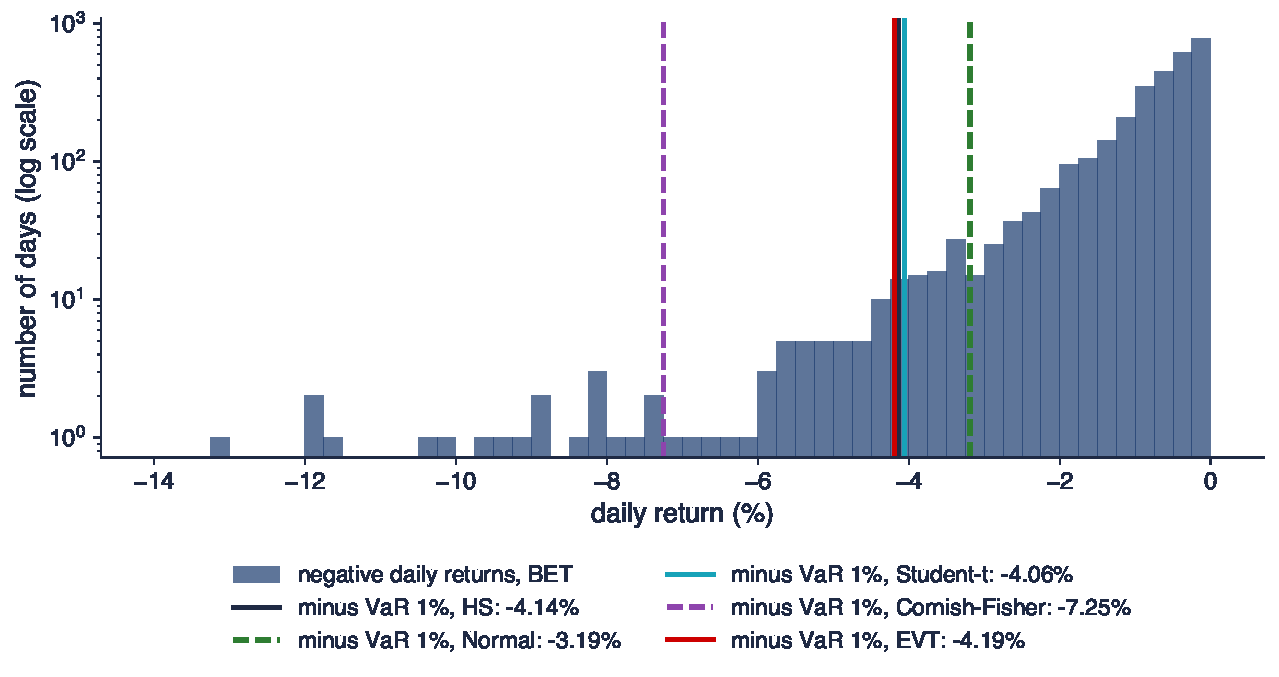
\includegraphics[width=0.96\textwidth,height=0.30\textheight,keepaspectratio]{ch10_sem_b1.pdf}
\end{center}
\vspace{-2mm}
\begin{center}
\scriptsize
\begin{tabular}{lrrrrr}
\toprule
& HS & Normală & Student-t & Cornish--Fisher & EVT \\
\midrule
VaR 1\% & $4{,}14$ & $3{,}19$ & $4{,}06$ & $7{,}25$ & $4{,}19$ \\
ES 2,5\% & $4{,}57$ & $3{,}21$ & $4{,}76$ & $7{,}93$ & $4{,}57$ \\
\bottomrule
\end{tabular}
\end{center}
\begin{itemize}
    \item $n = 6\,670$; $\hat\mu = 0{,}064$, $\hat\sigma = 1{,}40$; $S = -0{,}65$, $K = 11{,}1$; $\hat\nu = 2{,}43$; EVT: $u = 1{,}24\%$, $N_u = 667$, $\hat\xi = 0{,}23$
    \item VaR 1\% Normal este cu 23\% sub date; Cornish--Fisher ($z_{CF} = -5{,}23$) este mult peste toate celelalte
    \item Interpretare: raportăm valoarea istorică sau pe cea EVT (circa 4{,}14\% și 4{,}57\%), care sînt de acord; menționăm că distribuția Normală subestimează, iar Cornish--Fisher este în afara domeniului de valabilitate cu $K > 10$
\end{itemize}\sfmquantlet{Ch_10}{SFM_ch10_seminar}
\end{frame}

\begin{frame}{B2: TLV, SNP și Bitcoin [Propus]}
\itemsize{\footnotesize}
\begin{itemize}
\item \textbf{Întrebarea}: se păstrează ordinea metodelor găsită pentru BET la două acțiuni BVB și la Bitcoin? Model: B1.
\item \textbf{Date}: TLV și SNP din 2010 (TLV fără 30--31 mai 2016), Bitcoin din 2014; randamente logaritmice zilnice în \%
\item \textbf{Cerințe}
\begin{enumerate}
    \item Calculați VaR 1\% și ES 2,5\% pentru fiecare serie, cu cele cinci metode din B1.
    \item Calculați cu cît este VaR 1\% Normal sub VaR 1\% istoric.
    \item Raportați $\hat\nu$, $\hat\xi$ și excesul de boltire pentru fiecare serie.
    \item Interpretare: pentru care serie subestimează cel mai mult distribuția Normală VaR 1\%?
\end{enumerate}
\item \textbf{Raportați}: un tabel și două fraze
\item Notebook: secțiunea B2
\end{itemize}
\end{frame}

\ifsolutions
\begin{frame}{B2: rezolvare [Propus]}
\itemsize{\footnotesize}
\begin{center}
\scriptsize
\begin{tabular}{l|rrrrr|rrr|rr}
\toprule
& \multicolumn{5}{c|}{VaR 1\%} & \multicolumn{3}{c|}{ES 2,5\%} & & \\ & HS & N & t & CF & EVT & HS & N & EVT & abatere N & $K$ \\
\midrule
TLV & $5{,}11$ & $4{,}01$ & $4{,}63$ & $10{,}19$ & $4{,}90$ & $5{,}37$ & $4{,}03$ & $5{,}35$ & 22\% & ${13{,}5}$ \\
SNP & $4{,}29$ & $3{,}70$ & $4{,}26$ & $7{,}55$ & $4{,}38$ & $4{,}70$ & $3{,}72$ & $4{,}71$ & 14\% & ${8{,}9}$ \\
Bitcoin & $10{,}54$ & $7{,}99$ & $11{,}06$ & $18{,}89$ & $10{,}38$ & $10{,}84$ & $8{,}03$ & $10{,}90$ & 24\% & ${12{,}0}$ \\
\bottomrule
\end{tabular}
\end{center}
\begin{itemize}
    \item N: Normală, t: Student-t, CF: Cornish--Fisher; abatere N: cu cît este VaR 1\% Normal sub HS
    \item Ordinea din B1 se păstrează: distribuția Normală dă valori prea mici, CF mult prea mari, HS și EVT sînt apropiate; $\hat\nu$: TLV $3{,}44$, SNP $3{,}79$, Bitcoin $2{,}23$; $\hat\xi$: $0{,}26$, $0{,}22$, $0{,}12$
    \item Interpretare: Bitcoin (24\%) și TLV (22\%): cele mai groase cozi în raport cu varianța; SNP are cea mai mică abatere
\end{itemize}\sfmquantlet{Ch_10}{SFM_ch10_seminar}
\end{frame}
\fi

\begin{frame}{B3: backtesting pentru S\&P 500, an cu an [Rezolvat]}
\itemsize{\footnotesize}
\begin{itemize}
\item \textbf{Întrebarea}: pe care dintre două modele VaR 1\% l-ar fi penalizat o autoritate de supraveghere, an cu an, din 2015?
\item \textbf{Date}: S\&P 500 din 2000; prognoze pentru fiecare zi de la 2 ianuarie 2015
\item \textbf{Cerințe}
\begin{enumerate}
    \item Calculați VaR 1\% pe o zi prin simulare istorică pe ultimele 250 de zile.
    \item Calculați VaR 1\% pe o zi din GARCH(1,1)-t, reestimînd modelul la începutul fiecărui an pe toate datele anterioare.
    \item Numărați depășirile fiecărui model în fiecare an calendaristic și precizați zona Basel a fiecărui an.
    \item Aplicați testele Kupiec și Christoffersen pe întreaga perioadă.
    \item Interpretare: ce model ar fi penalizat o autoritate de supraveghere în 2022?
\end{enumerate}
\item \textbf{Raportați}: graficul, șase statistici cu p-valori și două fraze
\item Notebook: secțiunea B3
\end{itemize}
\end{frame}

\begin{frame}{B3: rezolvare [Rezolvat]}
\itemsize{\scriptsize}
\begin{center}
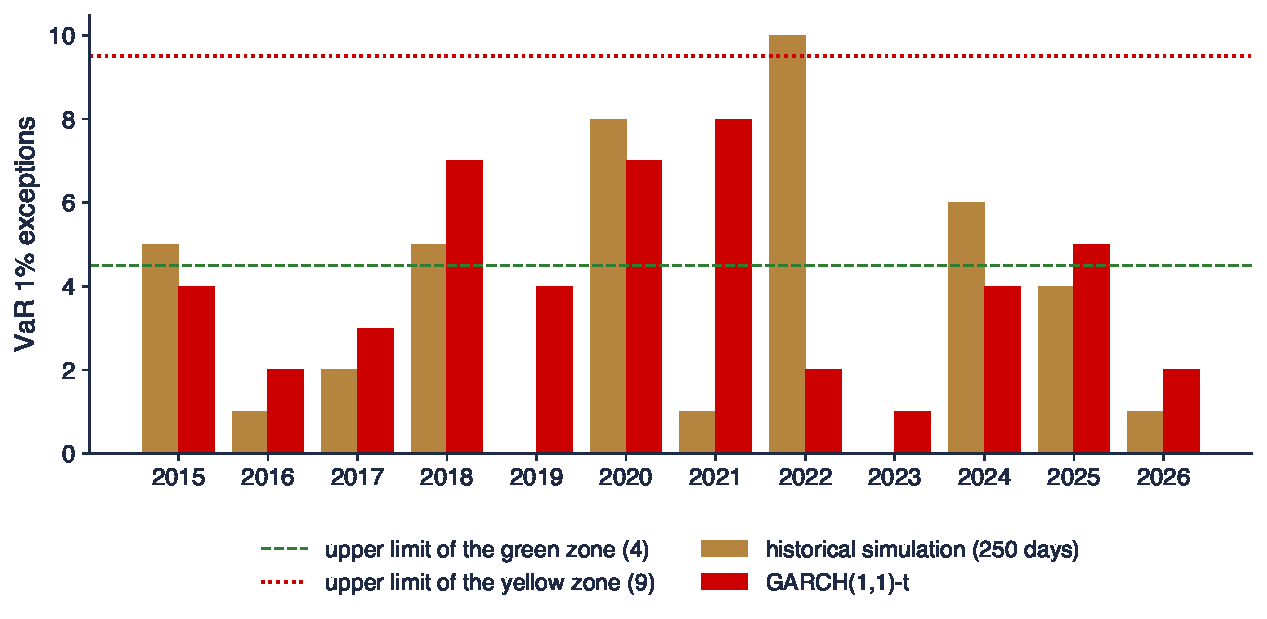
\includegraphics[width=0.96\textwidth,height=0.34\textheight,keepaspectratio]{ch10_sem_b3.pdf}
\end{center}
\vspace{-2mm}
\begin{center}
\scriptsize
\begin{tabular}{lrrrrrrr}
\toprule
& $n$ & $x$ & rata (\%) & $LR_{uc}$ (p) & $LR_{ind}$ (p) & $LR_{cc}$ (p) & ani roșii/galbeni \\
\midrule
HS 250 & 2\,944 & 43 & $1{,}46$ & $5{,}52$ (0{,}019) & $23{,}04$ ($<$\,0{,}001) & $28{,}56$ ($<$\,0{,}001) & 1/4 \\
GARCH-t & 2\,944 & 49 & $1{,}66$ & $10{,}94$ ($<$\,0{,}001) & $6{,}78$ (0{,}009) & $17{,}72$ ($<$\,0{,}001) & 0/4 \\
\bottomrule
\end{tabular}
\end{center}
\begin{itemize}
    \item Ambele modele sînt depășite prea des (așteptat circa 29{,}4); depășirile HS apar puternic grupat ($n_{11} = 7$, p ind.\ $<$\,0{,}001), cele GARCH-t mai puțin ($n_{11} = 4$)
    \item Interpretare: în 2022, HS a avut 10 depășiri (zona roșie), GARCH-t 2: fereastra lentă a fost penalizată cînd volatilitatea a crescut; GARCH-t a fost penalizat în anii mai liniștiți (2021: 8)
\end{itemize}\sfmquantlet{Ch_10}{SFM_ch10_seminar}
\end{frame}

\begin{frame}{B4: backtesting pentru BET și Bitcoin [Propus]}
\itemsize{\footnotesize}
\begin{itemize}
\item \textbf{Întrebarea}: se păstrează concluzia din B3 la BVB și pentru Bitcoin? Model: B3.
\item \textbf{Date}: BET din 2000, prognoze din 2015; Bitcoin din 2014, prognoze din 2016
\item \textbf{Cerințe}
\begin{enumerate}
    \item Calculați ambele prognoze VaR 1\% ca în B3.
    \item Numărați depășirile pe ani calendaristici și precizați zonele.
    \item Aplicați testele Kupiec și Christoffersen pe întreaga perioadă.
    \item Interpretare: ce model ați păstra pentru fiecare serie?
\end{enumerate}
\item \textbf{Raportați}: un tabel și două fraze
\item Notebook: secțiunea B4
\end{itemize}
\end{frame}

\ifsolutions
\begin{frame}{B4: rezolvare [Propus]}
\itemsize{\footnotesize}
\begin{center}
\scriptsize
\begin{tabular}{llrrrrrrr}
\toprule
& & $n$ & $x$ & rata (\%) & p POF & p ind. & p ac.c. & ani roșii/galbeni \\
\midrule
BET & HS 250 & 2\,926 & 43 & $1{,}47$ & 0{,}017 & 0{,}003 & $<$\,0{,}001 & 0/2 \\
 & GARCH-t & 2\,926 & 34 & $1{,}16$ & 0{,}391 & 0{,}371 & 0{,}464 & 0/3 \\
Bitcoin & HS 250 & 3\,914 & 40 & $1{,}02$ & 0{,}891 & 0{,}069 & 0{,}190 & 0/2 \\
 & GARCH-t & 3\,914 & 50 & $1{,}28$ & 0{,}094 & 0{,}672 & 0{,}226 & 0/5 \\
\bottomrule
\end{tabular}
\end{center}
\begin{itemize}
    \item BET: GARCH-t trece toate cele trei teste (rata 1{,}16\%); HS este depășit prea des, iar depășirile lui apar grupat
    \item Bitcoin: HS trece testele (rata 1{,}02\%); GARCH-t este la limită (1{,}28\%, p POF 0{,}094), cu 5 ani în zona galbenă
    \item Interpretare: păstrăm GARCH-t pentru BET și HS (sau FHS) pentru Bitcoin: cea mai bună metodă depinde de piață, deci fiecare model are nevoie de propriul backtesting
\end{itemize}\sfmquantlet{Ch_10}{SFM_ch10_seminar}
\end{frame}
\fi

\begin{frame}{B5: un portofoliu cu două acțiuni BVB [Rezolvat]}
\itemsize{\footnotesize}
\begin{itemize}
\item \textbf{Întrebarea}: cît reduce diversificarea între Banca Transilvania și OMV Petrom VaR 1\% și rezistă ea într-o criză?
\item \textbf{Date}: închiderile ajustate TLV și SNP din 2010, aliniate pe zilele comune; randamente simple în \%; ponderi 50/50
\item \textbf{Cerințe}
\begin{enumerate}
    \item Calculați VaR 1\% varianță--covarianță al portofoliului, cele două VaR individuale și beneficiul diversificării.
    \item Calculați VaR 1\% și ES 2,5\% istorice ale portofoliului.
    \item Calculați corelația din 2017 și din februarie--mai 2020, precum și dependența în cozi la $q = 5\%$ și $q = 1\%$.
    \item Estimați o copulă t și calculați VaR 1\% prin copulă, cu marginale empirice.
    \item Interpretare: de ce subestimează VaR varianță--covarianță riscul acestui portofoliu?
\end{enumerate}
\item \textbf{Raportați}: opt valori, graficul și două fraze
\item Notebook: secțiunea B5
\end{itemize}
\end{frame}

\begin{frame}{B5: rezolvare [Rezolvat]}
\itemsize{\scriptsize}
\begin{center}
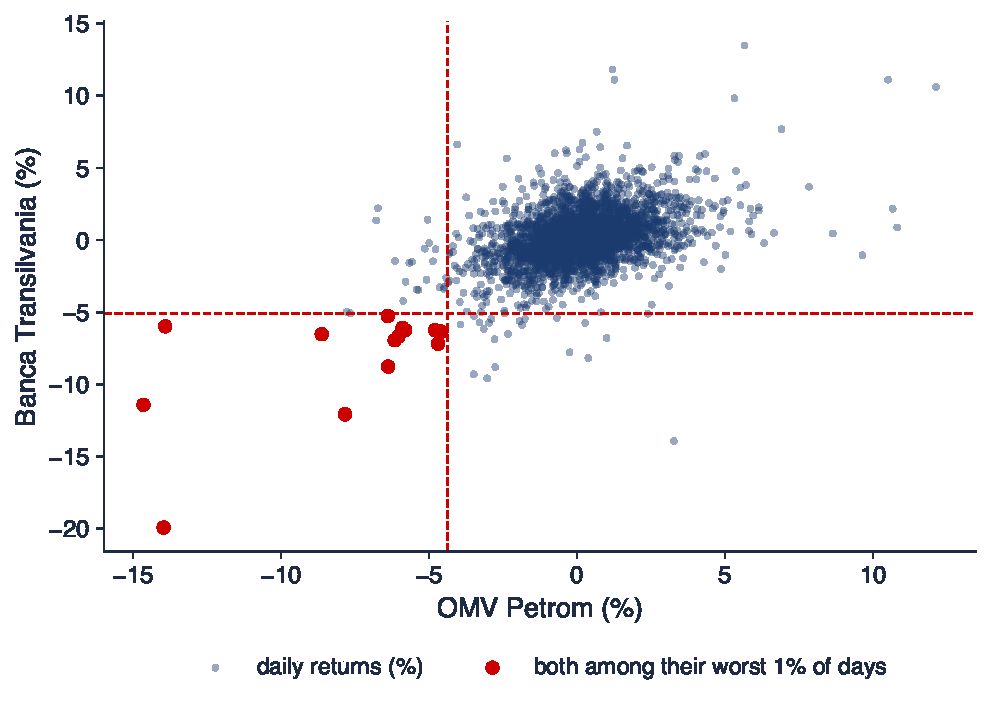
\includegraphics[width=0.96\textwidth,height=0.32\textheight,keepaspectratio]{ch10_sem_b5.pdf}
\end{center}
\vspace{-2mm}
\begin{itemize}
    \item $n = 3\,461$; $\hat\sigma$: TLV $1{,}84$, SNP $1{,}70$; $\hat\rho = 0{,}46$; $\sigma_p = 1{,}511$; VaR 1\%: TLV $4{,}17$, SNP $3{,}85$, portofoliu $3{,}41\%$; beneficiu 15\%
    \item Istoric: VaR 1\% $= 4{,}12\%$, ES 2,5\% $= 4{,}51\%$; copula t ($\hat\nu = 5{,}00$, $\lambda = 0{,}166$): VaR 1\% $= 3{,}96\%$
    \item Corelația: 2017 $0{,}32$, primăvara 2020 $0{,}69$; dependența în cozi $0{,}36$ ($q = 5\%$), $0{,}40$ ($q = 1\%$); zile comune în cel mai prost 1\%: 14, față de 0{,}35 la independență
    \item Interpretare: VaR Normal este cu 17\% sub cel istoric: ambele marginale au cozi groase, iar cele două acțiuni scad împreună în zilele cele mai proaste, cînd corelația este maximă
\end{itemize}\sfmquantlet{Ch_10}{SFM_ch10_seminar}
\end{frame}

\begin{frame}{B6: DAX și S\&P 500 [Propus]}
\itemsize{\footnotesize}
\begin{itemize}
\item \textbf{Întrebarea}: este copula Gaussiană suficient de bună pentru un portofoliu 50/50 DAX și S\&P 500? Model: B5.
\item \textbf{Date}: închiderile DAX și S\&P 500 din 2000, aliniate pe zilele comune; randamente simple în \%
\item \textbf{Cerințe}
\begin{enumerate}
    \item Calculați VaR 1\% și ES 2,5\% prin metoda varianță--covarianță și prin simulare istorică.
    \item Estimați copula Gaussiană și copula t și comparați-le prin statistica LR.
    \item Calculați VaR 1\% și ES 2,5\% prin copule, cu marginale empirice, pentru ambele copule.
    \item Interpretare: este copula Gaussiană suficient de bună pentru această pereche?
\end{enumerate}
\item \textbf{Raportați}: un tabel și două fraze
\item Notebook: secțiunea B6
\end{itemize}
\end{frame}

\ifsolutions
\begin{frame}{B6: rezolvare [Propus]}
\itemsize{\footnotesize}
\begin{center}
\footnotesize
\begin{tabular}{lrr}
\toprule
Metoda & VaR 1\% & ES 2,5\% \\
\midrule
varianță--covarianță & $2{,}72$ & $2{,}74$ \\
copula Gaussiană & $3{,}22$ & $3{,}34$ \\
copula t & $3{,}35$ & $3{,}51$ \\
simulare istorică & $3{,}36$ & $3{,}57$ \\
\bottomrule
\end{tabular}
\end{center}
\begin{itemize}
    \item $n = 6\,605$; $\hat\rho = 0{,}60$, $\hat\tau = 0{,}387$, $\rho$ al copulei $= 0{,}571$; copula t $\hat\nu = 3{,}00$, LR $= 611{,}4$ față de copula Gaussiană, $\lambda = 0{,}355$
    \item Copula t reproduce aproape exact VaR 1\% istoric; copula Gaussiană dă o valoare mai mică, iar VaR varianță--covarianță una și mai mică
    \item Interpretare: nu: două piețe dezvoltate cu ore de tranzacționare suprapuse au o dependență în cozi puternică ($\lambda = 0{,}355$), pe care doar copula t o surprinde
\end{itemize}\sfmquantlet{Ch_10}{SFM_ch10_seminar}
\end{frame}
\fi


%=============================================================================
\section{Partea C: întrebări deschise și critica unui răspuns AI}
%=============================================================================

\begin{frame}{C1: este ES 2,5\% la fel de mare ca VaR 1\%? [Propus]}
\itemsize{\footnotesize}
\begin{itemize}
\item \textbf{Întrebarea}: Basel a înlocuit VaR 1\% cu ES 2,5\% deoarece cele două sînt egale pentru randamente Normale; cît de apropiate sînt pe date reale și în crize?
\item \textbf{Date}: S\&P 500, DAX, BET, Bitcoin, TLV, SNP, BRD; modele: B1, A5
\item \textbf{Cerințe}
\begin{enumerate}
    \item Calculați raportul ES 2,5\% / VaR 1\% prin simulare istorică pe eșantionul complet al fiecărei serii.
    \item Calculați același raport pe cele 500 de zile care se încheie în martie 2009 și în mai 2020.
    \item Calculați raportul implicat de o distribuție Student-t estimată.
    \item Interpretare: este ES 2,5\% o regulă mai strictă decît VaR 1\% pe aceste piețe?
\end{enumerate}
\item \textbf{Raportați}: un tabel și un plan de proiect
\item Notebook: secțiunea C1
\end{itemize}
\end{frame}

\ifsolutions
\begin{frame}{C1: analiză de referință [Propus]}
\itemsize{\footnotesize}
\begin{center}
\scriptsize
\begin{tabular}{lrrrrr}
\toprule
& toate datele & 500 z. pînă la 3/2009 & 500 z. pînă la 5/2020 & Student-t & $\hat\nu$ \\
\midrule
S\&P 500 & $1{,}09$ & $0{,}97$ & $1{,}10$ & $1{,}14$ & $2{,}7$ \\
DAX & $1{,}01$ & $0{,}90$ & $1{,}26$ & $1{,}11$ & $3{,}1$ \\
BET & $1{,}10$ & $0{,}89$ & $1{,}06$ & $1{,}17$ & $2{,}4$ \\
Bitcoin & $1{,}03$ & -- & $1{,}21$ & $1{,}21$ & $2{,}2$ \\
TLV & $1{,}05$ & -- & $1{,}12$ & $1{,}09$ & $3{,}4$ \\
SNP & $1{,}10$ & -- & $1{,}09$ & $1{,}07$ & $3{,}8$ \\
BRD & $1{,}04$ & -- & $1{,}09$ & $1{,}05$ & $4{,}7$ \\
\bottomrule
\end{tabular}
\end{center}
\begin{itemize}
    \item Distribuția Normală: $1{,}005$; datele: de la $0{,}89$ la $1{,}26$; Bitcoin și acțiunile BVB nu au date înainte de 2009
    \item Raportul poate fi sub 1 (ferestrele care se încheie în 2009): o pierdere foarte mare împinge VaR 1\% în sus mai mult decît media ES 2,5\%
    \item Designul proiectului: rapoarte pe ferestre mobile pentru multe active, intervale bootstrap (raportul este zgomotos), legătura cu indicele de coadă $\xi$ (\sfmchlink{https://danpele.github.io/SFM/RO/Cursuri/capitol5_cozi_groase_evt.pdf}{Capitolul 5}) și capitalul cerut de fiecare regulă
\end{itemize}\sfmquantlet{Ch_10}{SFM_ch10_seminar}
\end{frame}
\fi

\begin{frame}{C2: verificați un răspuns AI [Propus]}
\itemsize{\scriptsize}
\begin{itemize}
    \item Un student a cerut unui asistent AI să rezume riscul BET în ultimele 500 de zile. Răspunsul:
    \item \aiprompt{(a) VaR 99\% al BET este -2{,}93\%.}
    \item \aiprompt{(b) ES este întotdeauna cel puțin la fel de mare ca VaR, deci ES 2,5\% este peste 2{,}93\%.}
    \item \aiprompt{(c) VaR 1\% pe 10 zile este 10 x 2{,}93 = 29{,}3\%.}
    \item \aiprompt{(d) Cu 8 depășiri în 250 de zile, p-valoarea Kupiec este 0{,}005, dar modelul rămîne în zona verde.}
    \item \aiprompt{(e) VaR este subaditiv, deci VaR-ul unui portofoliu nu depășește niciodată suma VaR-urilor componentelor.}
    \item \aiprompt{(f) Dacă depășirile apar grupat, testul Christoffersen poate respinge modelul chiar dacă numărul lor este corect.}
    \item Cerințe
    \begin{itemize}
        \item 1. Pentru fiecare afirmație, precizați dacă este corectă; dacă nu este, formulați afirmația corectă și, acolo unde se poate, dați valoarea corectă din notebook (secțiunea C2).
        \item 2. Raportați: o listă de șase verdicte, fiecare cu un rînd de justificare.
    \end{itemize}
\end{itemize}
\end{frame}

\ifsolutions
\begin{frame}{C2: rezolvare [Propus]}
\itemsize{\footnotesize}
\begin{itemize}
    \item (a) Greșit de două ori: nivelul este probabilitatea cozii (VaR 1\%), iar VaR este o pierdere, un număr pozitiv: VaR 1\% $= 2{,}93\%$
    \item (b) Greșit: $\mathrm{ES}_\alpha \ge \mathrm{VaR}_\alpha$ doar la același nivel; aici ES 2,5\% $= 2{,}69\%$ este sub VaR 1\% (A3)
    \item (c) Greșit: regula rădăcinii pătrate a timpului dă $\sqrt{10} \times 2{,}93 = 9{,}25\%$ și chiar și aceasta este valabilă doar pentru randamente Normale i.i.d.
    \item (d) Greșit: 8 depășiri înseamnă zona galbenă (adaosul 0,75); $LR_{uc} = 7{,}73$ respinge și el modelul
    \item (e) Greșit: VaR poate să nu fie subaditiv (cele două obligațiuni din A4); ES este măsura coerentă
    \item (f) Corect: aceasta este componenta de independență a testului de acoperire condiționată (A6)
\end{itemize}\sfmquantlet{Ch_10}{SFM_ch10_seminar}
\end{frame}
\fi


%=============================================================================
\section{Încheiere}
%=============================================================================

\begin{frame}{Idei de reținut}
\itemsize{\small}
\begin{itemize}
    \item VaR 1\% $= -q_{1\%}$, o pierdere pozitivă; ES 2,5\% face media celor mai proaste 2,5\% dintre zile; ES $\ge$ VaR doar la același nivel
    \item Pe date reale, metoda Normală subestimează VaR; Cornish--Fisher nu funcționează pentru boltire mare; HS și EVT sînt de acord la 1\%
    \item Backtesting-ul are nevoie de două verificări: numărul depășirilor (Kupiec) și independența lor (Christoffersen)
    \item Diversificarea este cea mai slabă în crize: corelația și dependența în cozi cresc împreună
    \item Un răspuns AI este o ciornă: verificați semnul și nivelul VaR, regula pentru orizont și zona Basel
\end{itemize}
\end{frame}

\begin{frame}{După seminar}
\itemsize{\small}
\begin{itemize}
    \item Cursul 10 dezvoltă fiecare temă de azi: definițiile și coerența, metodele de estimare, VaR condiționat, portofoliile și copulele, backtesting-ul
    \item Încercați cerințele [Propus] în notebook; rezolvările se discută la seminar
    \item C1 poate deveni un proiect de echipă: rapoarte pe ferestre mobile, intervale bootstrap, capitalul cerut de fiecare regulă
    \item Lectură: \refFHH, cap.~16; exerciții în \refBHL, cap.~16; \refQRM, cap.~2
\end{itemize}
\end{frame}


%=============================================================================
\section{Bibliografie}
%=============================================================================

\begin{frame}{Bibliografie}
\itemsize{\tiny}
\begin{itemize}
    \item Acerbi, C., Tasche, D. (2002). \href{https://doi.org/10.1016/S0378-4266(02)00283-2}{On the coherence of expected shortfall}. \textit{Journal of Banking \& Finance}, 26(7), 1487--1503.
    \item Artzner, P., Delbaen, F., Eber, J.-M., Heath, D. (1999). \href{https://doi.org/10.1111/1467-9965.00068}{Coherent measures of risk}. \textit{Mathematical Finance}, 9(3), 203--228.
    \item Basel Committee on Banking Supervision (1996b). \href{https://www.bis.org/publ/bcbs22.htm}{Supervisory framework for the use of ``backtesting'' in conjunction with the internal models approach to market risk capital requirements}. Bank for International Settlements.
    \item Borak, S., Härdle, W.K., López-Cabrera, B. (2013). \href{https://doi.org/10.1007/978-3-642-33929-5}{\textit{Statistics of Financial Markets: Exercises and Solutions}}, 2nd ed. Springer.
    \item Christoffersen, P.F. (1998). \href{https://doi.org/10.2307/2527341}{Evaluating interval forecasts}. \textit{International Economic Review}, 39(4), 841--862.
    \item Cornish, E.A., Fisher, R.A. (1938). \href{https://doi.org/10.2307/1400905}{Moments and cumulants in the specification of distributions}. \textit{Revue de l'Institut International de Statistique}, 5(4), 307--320.
    \item Demarta, S., McNeil, A.J. (2005). \href{https://doi.org/10.1111/j.1751-5823.2005.tb00254.x}{The t copula and related copulas}. \textit{International Statistical Review}, 73(1), 111--129.
    \item Franke, J., Härdle, W.K., Hafner, C.M. (2019). \href{https://doi.org/10.1007/978-3-030-13751-9}{\textit{Statistics of Financial Markets: An Introduction}}, 5th ed. Springer.
    \item Kupiec, P.H. (1995). \href{https://doi.org/10.3905/jod.1995.407942}{Techniques for verifying the accuracy of risk measurement models}. \textit{Journal of Derivatives}, 3(2), 73--84.
    \item McNeil, A.J., Frey, R. (2000). \href{https://doi.org/10.1016/S0927-5398(00)00012-8}{Estimation of tail-related risk measures for heteroscedastic financial time series: an extreme value approach}. \textit{Journal of Empirical Finance}, 7(3--4), 271--300.
    \item McNeil, A.J., Frey, R., Embrechts, P. (2015). \href{https://press.princeton.edu/books/hardcover/9780691166278/quantitative-risk-management}{\textit{Quantitative Risk Management: Concepts, Techniques and Tools}}, revised ed. Princeton University Press.
\end{itemize}
\end{frame}

\end{document}
